\documentclass[11pt,a4paper]{article}
\usepackage[T1]{fontenc}
\usepackage[utf8]{inputenc}
\usepackage{lmodern}
\usepackage{microtype}
\usepackage[margin=27mm,headheight=14pt]{geometry}
\usepackage{amsmath,amssymb,amsthm,mathtools}
\usepackage{booktabs,longtable,tabularx,array}
\usepackage{enumitem}
\usepackage{xcolor}
\usepackage{graphicx}
\usepackage{tikz}
\usetikzlibrary{arrows.meta,positioning,calc}
\usepackage{listings}
\usepackage{fancyhdr}
\usepackage{hyperref}
\usepackage[nameinlink,noabbrev]{cleveref}
\definecolor{ink}{HTML}{17324D}
\definecolor{teal}{HTML}{136B73}
\definecolor{shade}{HTML}{F1F5F8}
\hypersetup{colorlinks=true,linkcolor=ink,citecolor=teal,urlcolor=teal,
 pdftitle={Marked parallelity interfaces and certified handlebody cores},
 pdfauthor={ProveIt research programme; prepared with ChatGPT},
 pdfsubject={Compressed normal topology and exact sector decomposition}}
\pagestyle{fancy}
\fancyhf{}
\fancyhead[L]{\small\textsc{ProveIt / Unknot Recognition}}
\fancyhead[R]{\small Marked parallelity interfaces}
\fancyfoot[C]{\thepage}
\setlength{\parskip}{3pt}
\setlength{\emergencystretch}{2em}
\setlist{topsep=4pt,itemsep=3pt,parsep=0pt}
\newtheorem{theorem}{Theorem}[section]
\newtheorem{lemma}[theorem]{Lemma}
\newtheorem{proposition}[theorem]{Proposition}
\newtheorem{corollary}[theorem]{Corollary}
\theoremstyle{definition}
\newtheorem{definition}[theorem]{Definition}
\newtheorem{remark}[theorem]{Remark}
\newtheorem{question}[theorem]{Research question}
\newcommand{\N}{\mathbb N}
\newcommand{\Z}{\mathbb Z}
\newcommand{\Q}{\mathbb Q}
\newcommand{\R}{\mathbb R}
\newcommand{\F}{\mathbb F}
\newcommand{\code}[1]{\texttt{#1}}
\newcommand{\cut}{\mathbin{\backslash\!\backslash}}
\newcommand{\per}{\operatorname{per}}
\newcommand{\supp}{\operatorname{supp}}
\newcommand{\poly}{\operatorname{poly}}
\newcommand{\bits}{\operatorname{bits}}
\newcolumntype{Y}{>{\raggedright\arraybackslash}X}
\lstset{basicstyle=\small\ttfamily,breaklines=true,columns=fullflexible,
 keepspaces=true,frame=single,rulecolor=\color{black!15},
 backgroundcolor=\color{shade},xleftmargin=3pt,xrightmargin=3pt,
 aboveskip=9pt,belowskip=9pt,showstringspaces=false}

\begin{document}
\hypersetup{pageanchor=false}
\begin{titlepage}
\vspace*{9mm}
{\color{teal}\large\textsc{ProveIt research memorandum}\par}
\vspace{10mm}
{\color{ink}\huge\bfseries Marked Parallelity Interfaces\par
 and Certified Handlebody Cores\par}
\vspace{6mm}
{\Large Polynomial local topology and exact sector decomposition\par
 for the unknot-recognition programme\par}
\vspace{11mm}
{\large Prepared for Vladimir Reshetnikov and the ProveIt project\par}
{\normalsize Research and implementation developed with ChatGPT\par}
\vspace{4mm}
{12 October 2026\par}
\vspace{10mm}
\begin{abstract}
The present contribution addresses two explicit bottlenecks in compressed
unknot recognition.  First, a normal cut already has a source-certified
parallelity bundle and a complementary core of at most $30T$ handles, but
component profiles alone do not determine its attaching surfaces.  We recover
cyclic boundary words, old-boundary gaps, and fibre transitions using two
additional compressed orbit queries.  Maximal proper runs of core ports are
disk interfaces; a complete marked boundary circle is an annular interface.
We combine this information with geometric co-core slides and raw handle
cancellation.  Saturating occurrence counts at two preserves every admissible
raw pivot.  In the square, genus-zero case, a source leaf order is complete
for the entire raw cancellation class, and an explicit induction proves
that the exceptional core in every Fibonacci layered-torus fixture is a ball.
Successful certificates give the exact handlebody census of the whole supplied
cut, including binary multiplicities, without constructing its individual pieces.

Second, we split a supplied quadrilateral-sector matching space into its finest
coordinate factors.  Although canonical triangle minima can mix those factors,
nonnegative vertex-link Euler characteristics force the global normalized Euler
maximum to occur in a single factor.  Complete standard-ray enumeration requires
a coarser interaction decomposition.  A genuine solid-torus counterexample
separates these two statements.  Another genuine family reduces the maintained
global subset iterator from exponentially many candidate solves to linearly
many local solves, with polynomial source preparation and verification.

The deliverable includes additive Python implementations, separate checkers,
exact source fixtures, adversarial tests, independent Regina comparisons, and
reproduction scripts.  These are local algorithmic and geometric results.
They do not establish a quasi-polynomial bound for the complete recognizer:
useful-surface coverage, patterned-state transport, and global search bounds
remain explicit research obligations.
\end{abstract}
\vfill
\noindent\small\textbf{Audited source.}
\url{https://github.com/VladimirReshetnikov/ProveIt}\par
\noindent\small\texttt{d2c5e1707fe783bbed06743ac732d70d83e6f27b}\par
\noindent\small\textbf{Delivery status.} Additive research contribution for review and
integration; no repository publication is part of this delivery.
\end{titlepage}
\hypersetup{pageanchor=true}

\tableofcontents
\newpage

\section{Research position and scope}
\label{main:position}

The appropriate next step is to make compressed geometric information usable
by an exact topological consumer.  The audited repository already counts and
classifies normal-surface components, reconstructs actual cut cells and their
boundaries, and extracts the full source parallelity bundle in handle indices
zero, one, and two.  It also retains the geometrically attached exceptional
core.  Replacing that construction with a prism-only approximation would lose
information and undo an improvement already present in the source.

The missing information addressed here is smaller and more specific.  A list
of ports belonging to a base component gives membership, but it does not say
which ports are consecutive, whether old boundary separates them, or whether
they occupy a complete boundary circle.  Those distinctions decide whether
the interface with the core is a disk or an annulus.  Once they are available,
the existing geometric core can support a conservative, independently checked
handlebody classifier.  A separate source-coordinate decomposition reduces
some of the search needed to find candidate surfaces in the first place.

\subsection{What is new here, what is inherited, and what is open}

\begin{table}[htbp]
\centering\small
\begin{tabularx}{\textwidth}{@{}p{.23\textwidth}Yp{.18\textwidth}@{}}
\toprule
Topic & Precise status in this contribution & Classification\\
\midrule
Binary orbit computation & Polynomial weighted AHT and the maintained
suffix-fold bound are used with attribution. & Inherited\\
Source parallelity & Complete bases, fibre charts, at most $30T$ core handles
and $66T$ ports already exist. & Inherited\\
Marked cyclic interface & Two source-derived queries recover maximal
attachment intervals and full marked circles, with independent replay. & New operator and proofs\\
Geometric core cancellation & Raw co-core counts admit exact saturation;
source leaf elimination becomes a certified geometric ball test. & New geometric application\\
Layered cores & An explicit all-size source calculation gives a ball core
for every positive multiple of the Fibonacci fixture. & New family theorem\\
Sector factors & Finest matching blocks, Euler localization, standard
interaction clusters, and a geometric separation family. & New source-level development\\
Complete recognition & No bound on useful candidate coverage, all inherited
patterns, or all hierarchy states is proved. & Open\\
\bottomrule
\end{tabularx}
\caption{The novelty claim is relative to the pinned ProveIt source.  Classical
linear algebra, handle theory, and orbit algorithms are not claimed as new.}
\label{main:status-table}
\end{table}

The permanent-one criterion for raw positive elimination already appears in
report~56.  Its new role here is geometric: raw occurrences are authenticated
intersections with a co-core system, and the positive update is realized by
actual disk slides.  An abstract presentation simplifier is not substituted
for a three-manifold proof.  Likewise, the polynomial control of dense weight
runs is already proved in \code{synthesis/suffix\_folds.tex}; the sharper
sparse-mark bound and explicit selector accounting below assemble the bounds
needed by the new interface, rather than purporting to discover weighted AHT.

\subsection{Relationship to the quasi-polynomial programme}

We use \emph{quasi-polynomial} in its usual broad sense
$\exp((\log n)^{O(1)})$.  The stronger target $n^{O(\log n)}$ is
$\exp(O((\log n)^2))$; these formulations should not be conflated.
Lackenby's March 2021 lecture handout announces
$2^{O((\log n)^3)}$ for diagrams with $n$ crossings\cite{Lackenby2021}.
The July 2026 manuscript gives a new hierarchy-based recognition algorithm;
its Section~9 explicitly separates iteration counting from an analysis of all
step costs\cite{Lackenby2026}.  We do not infer a checked implementation or a
complete complexity proof for ProveIt from an announced bound.

Our local bit-polynomial results are compatible with either target.  They
eliminate dependence on the \emph{numerical multiplicity} of a supplied cut in
the accepted class, and the sector result replaces total matching dimension
by local block dimensions when splitting occurs.  Neither statement bounds
the number of candidates or the number and size of future patterned states.
The difference is consequential: polynomial verification of exponentially
many candidate certificates still permits exponential search.

\section{Input model and the authenticated geometric interface}
\label{main:model}

The runtime contract is a finite, connected, compact, orientable triangulated
three-manifold $M$ with one torus boundary, supplied by source face pairings,
and an admissible integral standard normal vector
$x\in\N^{7T}$.  The surface $S(x)$ may be empty, disconnected, or one-sided.
The source validator checks the relevant manifold links, face inverses,
matching equations, and quadrilateral constraints.  The exact cut is denoted
$M\cut S$: equivalently, remove the interior of a sufficiently small regular
neighbourhood and round its corners.  One-sided surfaces use their actual
normal interval bundle, not two fictitious orientable copies.

Put
\[
 D=\sum_i x_i,\qquad B=1+\lceil\log_2(D+1)\rceil.
\]
The coordinates have $O(TB)$ bits, and the face pairing has $O(T\log(T+1))$
bits.  We charge arithmetic on binary endpoints and weights; an operation on
a $B$-bit integer is not assigned constant cost.  The article uses $n$ only
for original diagram size and $T$ for the triangulation under discussion.
No unproved bound relating a later hierarchy triangulation to $n$ is hidden
by switching those parameters.

\subsection{The inherited source theorem}

The following is the precise established input to the new geometric arguments.
It is proved in the audited source's parallelity chapter and its raw cut-cell
construction\cite{ProveIt2026}.

\begin{proposition}[Source parallelity contract, inherited]
\label{main:source-contract}
The supplied cut decomposes into an embedded interval bundle $\mathcal B$
over a possibly disconnected compact surface $B_0$ and a complementary
geometric handle core $K$.  There is a marked subset $A\subseteq\partial B_0$
such that
\[
 K\cap\mathcal B=p^{-1}(A),\qquad
 (h_0(K),h_1(K),h_2(K),h_3(K))
       \leq(6T,8T,12T,4T)
\]
coordinatewise.  The packet has $O(T)$ source charts, including the complete
core attaching cycles, fibre reversals, and at most $P\leq66T$ singleton core
ports.  Its base representation has at most $17T$ polygon families, $44T$
gluing families, and $68T$ side slots, with binary rank intervals.
\end{proposition}

The selected handles are the chambers between consecutive identical normal
disks, the internal-face strips between consecutive parallel arcs, and the
gaps between consecutive intersections on an interior edge.  The complete
base uses truncated triangles and quadrilaterals, rectangles, and edge-link
polygons.  Its gluing includes every selected zero--one, zero--two and
one--two contact.  Omitting the last two kinds would invalidate the embedding
and intersection assertion.  The exceptional lower-index attachments stay
entirely in $K$; they are not group relators detached from source charts.

Four existing compressed queries determine the base-component profiles,
actual boundary counts, orientability, and port membership.  They also check
\begin{equation}
\label{main:euler-identity}
 \chi(M\cut S)=\chi(K)+\chi(B_0)-\chi(A).
\end{equation}
A base profile containing any port has multiplicity one.  Unported components
may have large binary multiplicity.  This distinction is necessary when a
finite attachment graph is formed: it is incorrect to turn a profile of
multiplicity $m$ into a single ordinary vertex.

\subsection{Trust boundary and certificate meaning}

The source-level geometric result in Proposition~\ref{main:source-contract}
is a mathematical dependency.  The existing checker reconstructs its charts
from the raw cut-cell reference model using a different extraction route.
The new checkers authenticate their inputs through that checker.  Thus an
accepted certificate depends on the source theorem and the correctness of
the small verifier stack, as any certified numerical implementation depends
on its trusted primitives.  It is not a formal proof in Lean, Coq, or Isabelle.

The standalone core helper has a narrower contract: its caller must already
have authenticated the geometric charts.  A dictionary of integer words with
the same occurrence matrix is insufficient.  The whole-cut wrapper supplies
the missing authentication.  A \code{COMPLETE} result from that wrapper means
an exact census of handlebodies in the \emph{supplied cut}.  It carries no
standalone knot verdict.  In particular, one ball component in a multi-component
cut does not establish that the original exterior is a solid torus.

\begin{figure}[htbp]
\centering
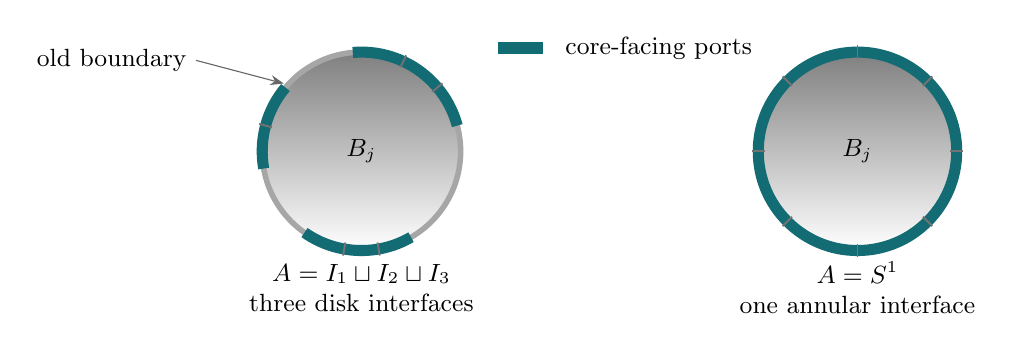
\begin{tikzpicture}[font=\small,scale=1.05]
  \fill[shade] (0,0) circle (1.2);
  \draw[black!35,line width=2pt] (0,0) circle (1.2);
  \foreach \a/\b in {15/95,140/190,235/300}{
    \draw[teal,line width=4pt] (\a:1.2) arc (\a:\b:1.2);
  }
  \foreach \a in {40,65,165,260,280}{
    \draw[black!55,line width=.7pt] (\a:1.12)--(\a:1.28);
  }
  \node at (0,0) {$B_j$};
  \node[align=center] at (0,-1.65) {$A=I_1\sqcup I_2\sqcup I_3$\\three disk interfaces};
  \draw[-{Stealth},black!60] (-2,1.1)--(-.94,.82);
  \node[align=right,anchor=east] at (-2,1.1) {old boundary};
  \begin{scope}[xshift=6cm]
    \fill[shade] (0,0) circle (1.2);
    \draw[teal,line width=4pt] (0,0) circle (1.2);
    \foreach \a in {0,45,90,135,180,225,270,315}{
      \draw[black!55,line width=.7pt] (\a:1.12)--(\a:1.28);
    }
    \node at (0,0) {$B_j$};
    \node[align=center] at (0,-1.65) {$A=S^1$\\one annular interface};
  \end{scope}
  \draw[teal,line width=4pt] (1.65,1.25)--(2.2,1.25);
  \node[anchor=west] at (2.35,1.25) {core-facing ports};
\end{tikzpicture}
\caption{Schematic base boundaries.  Subdividing a blue arc into source ports
does not subdivide its attaching disk.  If every boundary arc faces the core,
the complete vertical interface is an annulus.  For a disk base, the entire
right-hand bundle is a two-handle, as proved later.}
\label{main:interface-figure}
\end{figure}

\section{Ordered parallelity interfaces with polynomial encoded cost}
\label{int:section}

The source parallelity construction already retains the complete base surfaces
of the selected product handles, their fibre twisting, and a bounded collection
of source-labelled arcs where they meet the complementary core.  Its component
profiles record which ports belong to a base, but that set does not specify the
cyclic order of the ports on its boundary.  In particular, several successive
port rectangles can form one attaching disk.  Counting them as independent
attaching disks changes the topology of the proposed gluing.

This section supplies an exact ordered interface operator.  It reconstructs
the ported boundary circles, distinguishes a common endpoint from a nonempty
original-boundary gap, transports the local fibre charts, and groups the ports
into the actual connected attaching intervals and circles.  All of this uses
binary rank data.  The construction does not walk through the potentially
enormous collection of individual normal polygons.

The relevant predecessor is the source geometry in the repository's
\texttt{parallelity.tex}, together with its independently reconstructed
cut-cell reference~\cite{ProveIt2026}.  The orbit-counting engine is the
Agol--Hass--Thurston algorithm, abbreviated AHT~\cite{AHT2006}.  The results below
separate three points: the already established polynomial weighted AHT
operation, a sharper bound for sparse marked weights, and the new extraction
of ordered topological attachments.  No priority claim for sparse weighted
orbit computation is intended.

\subsection{The encoded marked-boundary problem}
\label{int:model}

\begin{definition}[Marked polygonal interval bundle]
\label{int:definition}
An encoded marked polygonal interval bundle consists of a compact, possibly
disconnected surface $B$, an interval bundle $E\to B$, and a polygon-family
description with the following properties.
\begin{enumerate}
\item Polygon copies are indexed by finite integer intervals whose endpoints
are written in binary.  Each family has an explicitly listed finite sequence
of sides and corners.
\item Glued side families have partial affine rank maps of slope $+1$ or
$-1$, an explicit permutation of their two endpoints, and a separate bit
specifying whether the interval fibre reverses.  These data describe genuine
surface and bundle gluings.
\item Exactly $P$ distinguished free edges are individually named by the
integers $0,\ldots,P-1$.  Each occurs at one specified rank and has a local
direction from endpoint zero to endpoint one.  Their union is denoted $A$.
Every other free edge has the single label ``original boundary.''
\end{enumerate}
The original-boundary label in this definition carries no additional marked
points, curves, slopes, or subdivisions that must be preserved.
\end{definition}

In the normal-cut application, the distinguished edges are the source core
ports.  The source constructor accepts its existing validated finite,
connected, compact, orientable triangulation with one torus boundary and an
admissible integral standard normal vector.  It allows empty, disconnected,
and one-sided cutting surfaces.  Its geometry has at most $66T$ ports, where
$T$ is the number of tetrahedra.  If $D$ is the number of normal disks, its
corner universe has at most $32D$ points and is represented by $O(T)$
families and side records~\cite{ProveIt2026}.

The separate fibre bit is essential.  An order-reversing map of a one-point
rank interval has the same point map as an order-preserving one.  Neither
that map nor the endpoint permutation alone specifies fibre transport.
The new construction retains all three pieces of information.

The output concerns precisely those boundary circles of $B$ that meet $A$.
It does not list every unported boundary circle.  Their number and the base
topology remain available from the existing base-profile construction.

\subsection{Dense weighted transport and the sharper sparse invariant}
\label{int:weights}

We first make the complexity accounting explicit.  This also corrects an
overly cautious reading of later repository passages that express their cost
only in terms of realized weighted partitions.  The preceding repository
section \texttt{suffix\_folds.tex} already gives a polynomial bound for those
partitions.  Classical weighted AHT is likewise polynomial
\cite[Theorem~16]{AHT2006}.  There is no missing general dense-weight theorem
at this stage of the source-cut calculation.

\begin{lemma}[The existing suffix-fold bound]
\label{int:dense}
Let a valid forward AHT trace on $[0,N)$ start with at most $k$ pairings and
$R_0$ canonical constant weight runs.  Weights may be signed integer vectors.
After $\tau$ truncations the maintained suffix-only transport has at most
\[
                         R_0+2\tau
\]
weight runs.  If the trace has $E$ events, the total number of emitted
histogram blocks is at most
\[
                       E(R_0+2E+4k+2).
\]
For additive source intervals $[l_j,h_j)$ with weights $v_j$, every
intermediate coordinate has absolute value at most
\[
                  M=\sum_j(h_j-l_j)\lVert v_j\rVert_\infty.
\]
\end{lemma}

\begin{proof}
This is the suffix-specific argument already established in the
repository~\cite{ProveIt2026}; we recall it to specify exactly which native
operation is being bounded.  Suppose a translation truncation retains
$[0,C)$ and uses period $p$, with $b=C-p$.  Each removed point is sent to
\[
               \rho(x)=b+((x-b)\bmod p)\in[b,C).
\]
The retained prefix weights stay in place.  Let $J_-$ and $J_+$ be the old
interior changes strictly below and strictly above $C$, respectively.
Extend the removed suffix weight by zero.  Its discrete derivative is
supported at $C$, $N$, and $J_+$.  Summing over residues transports these
changes into one period.  Consequently every new interior change lies in
\[
                   J_-\cup\rho(J_+)\cup\{b,\rho(N)\}.
\]
The change at $C$, if there was one, disappears.  Thus at most two new
boundaries replace the vanished suffix boundaries, giving an increase of at
most two runs.

For a reversing truncation, the removed suffix is reflected into one
retained interval.  Its old interior changes are reflected individually;
only the two endpoints of the receiving interval can be additional changes.
The same bound follows.  Deletion, trimming, merger, and transmission leave
the point weights unchanged.  A static contraction retains an ordered
subsequence of the old values and cannot increase the number of runs.
Induction proves the first assertion.

No trace operation increases the number of pairings.  The complement of
their domains and ranges has at most $2k+1$ static gaps.  Intersecting these
gaps with a weight partition having $R$ runs produces at most $R+4k+2$
pieces, a deliberately conservative bound.  Summing over at most $E$
contractions and using $R\le R_0+2E$ gives the displayed output bound.

Finally, every original point contribution moves to exactly one current
representative or one already emitted orbit.  Taking absolute values before
adding the contributions proves the mass bound, including signed
cancellation.  Thus the growth in numerical values costs only logarithmically
many additional bits.  None of the quotient computations iterates over the
number of represented points.
\end{proof}

The useful strengthening for ordered interfaces is independent of the
number of truncations.

\begin{theorem}[Sparse additive orbit transport]
\label{int:sparse}
Supply an interval pseudogroup on $[0,N)$ by $k$ partial integral isometries,
and supply $K$ singleton weight atoms
\[
                        (x_j,w_j),\qquad w_j\in\mathbb Z^d.
\]
Locations may repeat and weights may have either sign.  Their weighted orbit
histogram is computable in time polynomial in
\[
                  k,\quad \log(N+2),\quad K,\quad d,
\]
and the input weight bit lengths.  Along a valid AHT trace, the active weight
function is supported at at most $K$ points and has at most $2K+1$ canonical
runs.  There are at most $K$ distinct nonzero output weight vectors, with at
most one further zero-weight row.

If the atoms have the unique scalar weights $w_j=2^j$, every active nonzero
value encodes a disjoint subset of the $K$ labels.  Every nonzero run is a
singleton, every nonzero histogram row has orbit multiplicity one, and all
mask values have at most $K$ bits.
\end{theorem}

\begin{proof}
Temporarily distinguish the atoms even when their numerical weights are
equal.  Maintain an allocation of the atoms that have not yet been emitted
to current universe points.  The weight at a point is the sum of its
allocated atoms.

Pairing deletion, trimming, periodic merger, and transmission do not move
the allocated atoms.  A translation truncation maps each atom in the deleted
suffix to its unique retained representative modulo the carrier period.
A reflection truncation maps each such atom to its unique reflected
representative.  When several atoms arrive at the same point, their weights
are added.  A static contraction emits all atoms at a deleted point as the
weight of that completed orbit, then reindexes the remaining points
monotonically.  No operation creates a second copy of an atom.

Induction proves that the atom subsets at all live points and all completed
orbits are pairwise disjoint.  Hence at most $K$ live points can have nonzero
weight.  A function supported on $K$ integer points has at most $K$ nonzero
singleton pieces and at most $K+1$ intervening zero pieces; coalescing equal
adjacent values can only improve this count.  Every nonzero final orbit
contains at least one atom, so there are at most $K$ such orbits and at most
$K$ nonzero histogram rows.  Arbitrarily many unmarked or cancelling orbits
share the single zero row.

Each weight coordinate is bounded in absolute value by
$\sum_j |(w_j)_i|$.  Its bit length is therefore at most the maximum input
coordinate bit length plus $\lceil\log_2(K+1)\rceil$ and a constant.
The maintained quotient/remainder and reflection operations process the
bounded run list with binary arithmetic.  A trace of $E$ events consequently
has polynomial weighted replay cost in the displayed parameters and $E$.
For example, a conservative implementation-level bound is
\[
             O\bigl(E(k+K)\log(k+K+2)+K\log(K+2)\bigr)
\]
arithmetic operations, with the vector dimension and actual integer operand
lengths included in the bit cost.  The polynomial classical AHT trace bound
then proves the claimed polynomial algorithm~\cite{AHT2006}.

For the unique scalar labels, sums of disjoint subsets of distinct powers
of two have no binary carries.  Distinct occupied points cannot carry the
same nonzero mask, because that would allocate one label to two points.
This also rules out a nonzero constant run of length greater than one and
rules out two distinct output orbits with the same nonzero mask.  The last
assertions follow.
\end{proof}

Thus the new bound can be recorded together with the existing one as
\[
                 R\le\min\{R_0+2\tau,\,2K+1\}.
\]
Its advantage here is that $K$ is the number of distinguished endpoints,
which is bounded by the source size.  It is not the number of normal disks.

\subsection{The label partitions in weighted selectors are polynomial too}
\label{int:selectors}

The existing complete base construction uses weighted least representatives
to mark individual quotient vertices and boundary components.  Its forward
implementation retains intervals of surviving original labels; its
independent checker restores deleted gaps backwards.  Both admit an explicit
bound that can be combined with Lemma~\ref{int:dense}.

\begin{proposition}[Tagged selector size]
\label{int:tagged}
Consider a complete monotone forward trace with $E$ events, at most $k$
pairings, and $R_0$ initial weight runs.  Let $G$ be the total number of
contracted static-gap intervals.  Then
\[
                 G\le(2k+1)E,
\]
and there are at most $1+G$ live original-label intervals at any time.
The forward tagged selector emits at most
\[
          E\bigl(R_0+2E+1+(2k+1)E+4k+2\bigr)
\]
raw tagged pieces.  Its coalesced output and its independent backward
verification have polynomial size and bit cost in the same parameters.
\end{proposition}

\begin{proof}
Initially the live original labels form one interval, or none when the
universe is empty.  Removing a contiguous interval of current ranks can
split one live original-label interval into two.  If instead it crosses
several live intervals, it deletes middle intervals and cuts only the two
end intervals, with no larger increase in their number.  Thus one removed
gap increases the live interval count by at most one.  Retaining a prefix
cannot increase it.  This proves the $1+G$ bound.  Each contraction has at
most $2k+1$ gaps, proving the bound on $G$.

At a contraction the emission routine intersects three ordered partitions:
the constant weight runs, the live source-label intervals in current-rank
coordinates, and the static gaps.  If their sizes are $R$, $L$, and $r$,
the common refinement contains at most $R+L+2r$ relevant pieces.  Substitute
\[
                R\le R_0+2E,\qquad
                L\le1+(2k+1)E,\qquad r\le2k+1
\]
and sum over at most $E$ contractions.  This gives the stated conservative
bound.  Sorting and coalescing these explicitly bounded pieces is
polynomial, and their endpoints remain binary source labels.

For the independent reverse construction, the selected tagged intervals
remain disjoint.  Inserting a removed gap has one insertion anchor, which
can split at most one currently selected interval.  Across all reverse
insertions there are at most $G$ such new splits beyond the pieces originally
recorded at contractions.  Truncations insert no selected points: a deleted
suffix contains no least original representative.  Binary gap insertion,
sorting, and coalescing therefore also have polynomial cost.  This argument
applies directly to the producer's live-label operations and the verifier's
separate backward reconstruction~\cite{ProveIt2026}.
\end{proof}

\begin{corollary}[Polynomial source-parallelity accounting]
\label{int:source-polynomial}
For the validated normal-cut source class with $T$ tetrahedra and $D$ normal
disks, the source-parallelity base construction, its tagged selectors, and
the ordered interface construction below have a polynomial-time realization
in $T$ and $\log(D+2)$.  No extra hypothesis about an uncontrolled number
of weighted or label partitions is required.
\end{corollary}

\begin{proof}
The source geometry has $O(T)$ records and binary rank endpoints.  Its
corner and polygon universes have sizes bounded by constant multiples of
$D$~\cite{ProveIt2026}.  The first two source-parallelity queries are the
weighted corner and boundary selectors.  Proposition~\ref{int:tagged}
bounds their outputs polynomially in their AHT traces.  The subsequent
mark-placement operation intersects their ordered representative intervals
with the $O(T)$ polygon-carrier intervals.  A common refinement of two
ordered interval families has polynomial size.  Hence the weights supplied
to the base-component and fibre-cover histograms have polynomially many
input intervals.  Lemma~\ref{int:dense} bounds both histograms and their
integer sizes.  Finally, Theorem~\ref{int:sparse} applies to the two ordered
interface queries.  Choosing classical polynomial AHT schedules for these
finitely many queries proves the corollary.
\end{proof}

The new ordered-interface implementation explicitly selects the original
AHT periodic-overlap threshold with \texttt{periodic\_rule='aht'} in both
queries.  The pre-existing source-parallelity implementation uses its
documented forward AHT engine, including its already justified stronger
Fine--Wilf merger.  The partition bounds above apply to either valid forward
schedule; their conversion to a worst-case input bound invokes the
polynomial trace bound for the chosen schedule.  In particular, the existing
phrases ``polynomial in the realized partitions'' need not be interpreted as
an additional unresolved source-parallelity hypothesis.  This is a
clarification of local encoded operations.  It gives no bound on the number
of cutting surfaces or hierarchy states that a complete recognizer must
discover.

\subsection{Two marked orbit queries recover the boundary words}
\label{int:construction}

Give every individual polygon corner its place in a single integer universe
$[0,N)$.  A gluing of polygon sides identifies their endpoint corners.  The
source rank maps and corner offsets express those identifications as partial
integer isometries.  Let $V$ denote the resulting interval equivalence
system.  Its orbits are the actual quotient vertices of the polygonal
surface.

For port $p$, introduce the two endpoint tokens
\[
                         e=2p,\qquad e=2p+1.
\]
Tokens are distinct names even when their corner points are identified or
are literally the same source corner.  Place the singleton scalar weight
$2^e$ at the corresponding corner.  The first query is the weighted orbit
histogram of $V$.  It records which distinguished endpoints are the same
surface vertex.  At a boundary vertex at most two port endpoints can occur,
because the boundary is a one-manifold.  Accordingly, each nonzero mask has
one or two bits and occurs once.

Next add to $V$ the endpoint identifications across every original-boundary
free edge, omitting every core-port edge.  Call the resulting system $G$.
It records connectivity along the boundary after the interiors of the port
edges have been removed.  Its marked components are intervals, including
the possible one-vertex interval between consecutive port edges.  Each has
exactly two endpoint tokens.

We do not need to query $G$ separately.  Instead, construct its two-sheeted
fibre cover $\widetilde G$ on $[0,2N)$.  Across an original corner gluing,
the source fibre bit either preserves or exchanges the sheets.  Across an
original-boundary free edge, the local polygon fibre chart preserves them.
The lifted token $(e,s)$ receives weight
\[
                              2^{2e+s},\qquad s\in\{0,1\}.
\]
The second query is the weighted histogram of $\widetilde G$.  Every marked
interval has two disjoint lifts, so the nonzero masks give a perfect
matching of the $4P$ lifted tokens.  If
\[
                            (e,0)\longleftrightarrow(f,b),
\]
the matching identifies the gap endpoints $e,f$ and its fibre reversal $b$.
The other lift must be
\[
                            (e,1)\longleftrightarrow(f,1-b).
\]
Both relations are checked; in particular $e\ne f$.

\begin{theorem}[Exact ordered interface extraction]
\label{int:ordered}
For an encoded marked polygonal interval bundle as in
Definition~\ref{int:definition}, two sparse weighted orbit queries determine,
for every boundary circle meeting $A$:
\begin{enumerate}
\item the cyclic order and local directions of all its port edges;
\item whether each intervening original-boundary gap is nonempty or consists
of a common vertex;
\item the fibre reversal along each gap in the specified endpoint charts;
\item the connected components of $A$, classified as intervals or whole
boundary circles, with the endpoint charts and fibre transport of every
interval component.
\end{enumerate}
The output has $O(P)$ records.  The queries have $2P$ and $4P$ singleton
tokens, respectively, and their weight partitions have at most $4P+1$ and
$8P+1$ runs.  The construction has polynomial encoded cost.  If the total
interval bundle is orientable, the fibre parity around every output
boundary circle is zero.
\end{theorem}

\begin{proof}
The first query computes actual corner equivalence and therefore tells
exactly which endpoint tokens are the same surface vertex.  Distinct
token names give disjoint bits, so their masks lose no endpoint information.
Unmarked vertices contribute only zero weight, regardless of their number.

Consider a boundary circle that contains at least one port.  Removing the
interiors of its port edges leaves a finite collection of compact intervals.
An interval can be a single vertex when two port edges are successive with
no intervening original-boundary edge.  Its two boundary incidences are the
two endpoint tokens that it carries.  The system $G$ gives exactly these
interval components: its corner relations identify surface vertices, and
its additional relations cross precisely the non-port boundary edges.
Unported boundary circles and interior vertices carry no endpoint labels.

An interval bundle over an interval is trivial.  In the two-sheet fibre
cover its two endpoint lifts therefore form two disjoint pairs.  The second
histogram recovers these pairs and the relative fibre chart.  This proves
the asserted endpoint matching and fibre reversal.  A gap is a single
vertex if and only if its two tokens belong to the same $V$-orbit.  Indeed,
the forward implication is immediate.  For the converse, a positive
original-boundary path beginning and ending at that vertex, in addition to
the two incident port-edge ends, would give more than two boundary
incidences there.  That contradicts the boundary one-manifold condition.

Join the recovered gap matching to the fixed port matching
$2p\leftrightarrow2p+1$.  Each endpoint is incident to one gap and one port,
so these alternating components are exactly the ported boundary circles.
Start each component at its least port, entering that port through its
endpoint zero.  Crossing a port in direction zero to one writes $p+1$;
crossing it in the other direction writes $-(p+1)$.  Crossing the following
gap determines the next port endpoint.  This produces a deterministic
signed cyclic word, up to the normalization just specified.  Every port
occurs exactly once in one such word, and there are exactly $P$ gaps
between consecutive ports in the aggregate.

Split a cyclic word at every nonempty original-boundary gap.  Its remaining
maximal runs are precisely the connected interval components of $A$.
If there is no such gap, the entire word is one circle component of $A$.
The local fibre transport along a port is trivial in its own polygon
chart.  Consequently, the XOR of the intervening gap bits gives the fibre
transport of each interval run, and the XOR around a cyclic word gives
its fibre monodromy.  When the total space $E$ is orientable, its interval
orientation character is $w_1(B)$.  The restriction of $w_1(B)$ to every
boundary circle vanishes, since that circle has an annular collar in $B$.
The total XOR around each boundary word is therefore zero.

Both orbit systems have a number of pairing families bounded by a constant
multiple of the input side and gluing records.  Doubling sheets doubles
the universe and only multiplies the number of families by a constant; it
does not expand the universe.  Theorem~\ref{int:sparse}, applied to $2P$
and $4P$ singleton tokens, gives the stated run and complexity bounds.
Decoding masks, forming the two matchings, traversing the $P$ port edges,
and splitting the words use polynomial work and $O(P)$ output records.
\end{proof}

\begin{corollary}[Source-size bound for ordered normal-cut interfaces]
\label{int:normal}
For the source normal-cut geometry, the reduced ordered core interfaces have
$O(T)$ records and can be computed in time polynomial in $T$ and
$\log(D+2)$, independently of the numerical normal multiplicities.
\end{corollary}

\begin{proof}
Substitute the source bounds $P\le66T$, $N\le32D$, and $O(T)$ polygon-side
records into Theorem~\ref{int:ordered}.  The geometry and the source-normal
validation are binary rank operations.  If $D=0$, there are no ports and the
empty interface follows directly from the source construction.
\end{proof}

\subsection{Attaching intervals, attaching annuli, and the exact invariant}
\label{int:attachments}

\begin{corollary}[Connected attachment types]
\label{int:attachment-types}
Suppose the output contains $a$ interval components and $c$ circle components
of $A$.  Then
\[
                \chi(A)=a,\qquad
                H_1(A;\mathbb Z)\cong\mathbb Z^c.
\]
In the orientable total-bundle setting, the interval-bundle attachment above
each component is a disk for an interval component and an annulus for a
circle component.  Adjacent source ports in one interval run form one
attaching disk.
\end{corollary}

\begin{proof}
A finite disjoint union of compact intervals and circles has the stated
Euler characteristic and first homology.  The restriction of any interval
bundle to an interval is a product, hence a disk.  On a boundary circle of
an orientable total bundle the fibre character is zero by
Theorem~\ref{int:ordered}; its vertical restriction is therefore an annulus.
The decomposition into components is the maximal-run decomposition already
proved, so the several rectangles over consecutive port arcs constitute
one connected disk, rather than separate attaching disks.
\end{proof}

The value $a$ agrees with the existing independently checked attachment
Euler characteristic, computed there as the number of quotient vertices
incident to core ports minus the number of core ports.  The new operator
retains the extra information that this Euler characteristic omits:
the number and identities of entire attaching circles, cyclic order,
individual interval membership, and fibre transport.

For example, the four-tetrahedron layered-meridian fixture has $15$ ports
but only three interval attachments.  An especially small annular
obstruction uses the two-tetrahedron layered source and the coordinate rows
\[
                (0,0,1,1,1,0,0),\qquad (1,1,1,1,0,0,0).
\]
Its source parallelity base is the edge-cap-only disk already described in
the repository's parallelity analysis~\cite{ProveIt2026}.  The new output
has the single word
\[
                         (1,2,3,4,5,6,7,8)
\]
and every following gap is a common vertex.  Thus $a=0$, $c=1$: its whole
base boundary is attached, and the corresponding vertical attachment is an
annulus.  A criterion that permits only attaching disks must exclude this
case.  It cannot replace the circle by eight independent disk attachments.

\subsection{Replication along a two-sided normal surface}
\label{int:replication}

The dependence on a large common multiplicity can be separated even more
strongly when a global coorientation is available.  The following statement
concerns the source decomposition itself, including its marked attachment
data; it is not merely a statement about the number of complementary
components.

\begin{theorem}[Positive-multiplicity replication]
\label{int:replication-theorem}
Let $F$ be a nonempty two-sided properly embedded normal surface with
admissible standard coordinate vector $x$ in a triangulated orientable
$3$-manifold satisfying the source contract.  Fix a global coorientation
on each component of $F$.  Write $K_x$ for the source complementary core
and $E_x\to B_x$ for its selected parallelity bundle.  For every integer
$m\ge1$, the standard normal surface with coordinates $mx$ admits the
following source-compatible description.
\begin{enumerate}
\item Its core is canonically identified with $K_x$ by the local handle
types and owners.  Source rank labels on its interface are obtained by
multiplying the corresponding local gap ranks by $m$.
\item In every product-handle family, whose local gap ranks have the form
$1\le r<md$ after replication, retain exactly the copies with $m\mid r$.
These copies form a union of complete bundle components.  Division of
their local ranks by $m$ identifies their polygonal bundle, including its
fibre charts and marked core attachment, with $E_x\to B_x$.
\item Every source core port belongs to this divisible-rank subbundle.
The remaining product handles form $m-1$ unported copies of $F\times I$,
with $m-1$ base copies of $F$.  If $F$ has $q$ connected components, this
means $(m-1)q$ additional connected unported bases.  Existing unported
components of $B_x$ are retained as well.
\item The reduced signed core-port words, the zero-or-positive
original-boundary gap indicators, and the fibre transport are unchanged
under the source identification.  In particular, the numbers and owner
incidences of attaching intervals and attaching circles are unchanged.
\end{enumerate}
The identification is by source family and local rank; the flattened
integer offsets and the numerical polygon-family IDs need not agree.
Topologically,
\[
 \operatorname{Cut}(M,mF)\cong
 \operatorname{Cut}(M,F)\;\sqcup\;
 \bigsqcup_{j=1}^{m-1}(F\times I).
\]
\end{theorem}

\begin{proof}
Choose a small two-sided normal collar of $F$ compatible with the fixed
coorientation.  Replace each local disk of $F$ by $m$ parallel disks in
that collar.  Face matching follows the old matching and the collar
coordinate, so this is an embedded normal representative of $mx$.
There are $m-1$ intervening product slabs over every component of $F$.
The remaining part of the complement is the old cut complement, with
its two cut sides shifted to the two exterior copies of the collar.
This proves the displayed topological decomposition.  We now verify
its stronger assertion about the specified source handles.

A local product handle lies between consecutive objects in one ordered
stack: parallel normal disks in a tetrahedron, parallel normal arcs in
a face, or normal intersection points on an interior edge.  If the old
stack has size $d$, its product ranks are $1,\ldots,d-1$.  Replication
replaces each old object by a block of $m$ objects.  The gap between
successive old blocks has rank $mr$, whereas an interior gap within a
block has rank not divisible by $m$.  Thus the divisible ranks are
exactly the old inter-block product handles.  If an old stack has
$d=1$, its source family was absent; the new ranks $1,\ldots,m-1$
are all nondivisible, as required.

This distinction is respected by every source gluing.  Expressed in
\emph{local gap ranks}, each gluing is
$r\mapsto\varepsilon r+c(x)$, where $\varepsilon\in\{1,-1\}$ and
$c(x)$ is a homogeneous integral linear combination of the relevant
normal disk counts.  For example, the prism-to-face maps are $r$,
$t_v+r$, or $t_v+q-r$, where $t_v$ is a triangle count and $q$ the
relevant quadrilateral count.  The prism-to-edge and face-to-edge maps
have the forms $t_v+r$, $w-t_v-r$, $r$, or $w-r$, where $w$ is an
edge weight; restrictions choose the appropriate family and interval.
These are gap ranks, so the $-1$ that occurs in a zero-based
\emph{disk} reflection has already been removed by the source conversion
to gap coordinates.  After replacing $x$ by $mx$, the offset becomes
$mc(x)$.  Hence divisible ranks glue only to divisible ranks, and
division by $m$ recovers every original gluing and its domain.  The
endpoint permutations and fibre-reversal bits depend on source
orientations and local disk types, which have not changed.  This proves
the asserted bundle identification, including local fibre charts.

The complementary source $0$-handles are the chambers at stack ends
and at changes of disk type.  Its $1$-handles are the corresponding
nonparallel face regions, its $2$-handles are the two exterior edge
gaps (or the sole gap for zero edge weight), and its $3$-handles are
the fixed interior vertex regions.  Positive scaling preserves all
zero-or-positive tests and disk-type supports.  Consequently their
types, owners, and attaching charts identify with those for $x$.
Each core-facing product port occurs at a transition rank such as
$t_v$, $t_v+q$, an arc count, or its complement in an edge weight.
These ranks are homogeneous in $x$, so all new port ranks are
divisible by $m$ and all old ports reappear at their rescaled ranks.
The possibly newly present product families with old stack size one
have no such interior divisible rank and contribute no core port.

The product handles at the nondivisible ranks fill precisely the
slabs inside the replicated collars.  The chosen global coorientation
orders the $m$ sheets consistently on each component of $F$, thereby
identifying the slabs as $F\times I$ with indices
$1,\ldots,m-1$.  A reversed local stack can exchange residue $s$
with $m-s$; this local effect does not exchange the globally indexed
slabs after the coorientation is used.  Their bases are the corresponding
copies of $F$ and their only vertical boundary lies over $\partial F$
in the original boundary of $M$.  None touches the source core.

Finally, the divisible-rank identification preserves all free-edge
labels, corner identifications, and fibre bits.  It therefore preserves
the two pairing problems used by Theorem~\ref{int:ordered} on every
ported component.  The reduced boundary words, their gap types, and
their attaching-component decomposition are identical after applying
the source identification.  This proves all four assertions.
\end{proof}

\begin{corollary}[Replication of a certified disk cut]
\label{int:replicated-disk}
If $F$ is a connected two-sided normal disk and its primitive source cut
has a valid handlebody census, then every positive multiple has the same
ported core and contributes $m-1$ additional unported balls.  In particular,
if the primitive cut is a single ball, the cut along $mF$ consists of
exactly $m$ balls.
\end{corollary}

\begin{proof}
Apply Theorem~\ref{int:replication-theorem} and use
$D^2\times I\cong D^3$ for the additional unported slabs.
\end{proof}

This theorem permits a future certificate format to retain a primitive
interface proof and a binary replication factor, once a source-bound
coorientation certificate has been checked.  The delivered implementation
still runs its general compressed queries on the supplied vector; it does
not use such a replication shortcut.  The coorientation hypothesis is
substantive: for a one-sided component the local sheet order can reverse
around a loop, and the asserted list of $m-1$ copies of $F$ does not follow.
The general ordered-interface operator itself remains valid in that case.

For the layered-meridian experiments below, the theorem proves independence
of the positive scalar $m$ once the primitive disk and its source interface
have been certified.  It does not prove an interface formula for all
numbers of layers.  In particular, the observed formulas for the number
of primitive ports and attaching intervals as the layer count varies
remain finite experimental observations here; no induction establishing
an all-layer primitive-interface theorem is claimed.


\subsection{Source-bound certificates and implementation contract}
\label{int:certificates}

The producer is
\texttt{normal\_parallelity\_boundary\_words}; the independently implemented
checker is \texttt{verify\_parallelity\_boundary\_words}.  The result retains
the source port records, including their core-handle owners, and contains
the following finite data.
\begin{itemize}
\item Each gap specifies its two endpoint token IDs, whether original
boundary is present, and its fibre reversal.  Endpoints are ordered by ID.
\item Each ported boundary circle contains its signed word, the corresponding
list of following gap IDs, and the whole-core-circle indicator.
\item Each connected attachment contains its interval-or-circle type, its
signed subword, and, for an interval, its entry and exit tokens and fibre
transport.  A least port ID serves as an anchor for joining it to the
existing base profile whose port mask contains that ID.
\end{itemize}

All ports in one connected attachment belong to the same base component.
A base profile containing a port has multiplicity one in the existing
source classification.  Thus the anchor joins the ordered interface to
the base topology without making any choice among repeated unported
components.

The certificate has schema
\texttt{parallelity-boundary-words-v1}.  It binds the input fingerprint,
the proposed interface, the weighted vertex-partition proof, and the
weighted gap-cover proof.  Verification reconstructs the parallelity
geometry through the separate raw-cut-derived reference.  It independently
forms the two pairing systems, checks the supplied AHT traces and weights,
and reconstructs the proposed words and connected attachments.  It does not
import the producer's query builder, mask decoder, traversal routine, or
discovery scheduler.

When $P=0$, the output is the empty interface.  Both proof fields are
explicitly null; neither orbit query is run.  The checker reconstructs the
source and verifies the absence of ports, so this shortcut does not rely
on a caller assertion.  It says nothing about the number of unported base
boundary circles, which this API has not been asked to enumerate.

A discovery-cycle limit is shared by the two queries.  Exhaustion returns
an inconclusive status without an interface or certificate.  A verification
operation limit counts the two supplied ordinary traces.  Cooperative
cancellation propagates through both paths.  The operation returns geometric
information about the supplied source and cutting vector; it does not
itself issue a knot verdict.

\subsection{Independent finite checks and binary scaling}
\label{int:evidence}

The added test module passed all eight test methods in the recorded run.
It covers $193$ source/vector cases: all $157$ saved native source cases,
$16$ layered-meridian cases, eight one-sided cases, and twelve source
relabellings.  Of these, $182$ are compared with a literal expanded oracle.
That oracle expands the actual free polygon edges, identifies corner fibre
charts with a parity union-find, and walks each old-boundary edge one at a
time.  It separately computes connected components using only the core
edges, rather than reusing the producer's maximal-word-run routine.  Eleven
very large native cases use compressed independent source replay and the
attachment-Euler and base-profile checks instead of exceeding the literal
oracle's point cap.

Further tests reject altered source fingerprints, core owners, signed
words, zero-gap flags, fibre bits, endpoint masks, and attachment types.
They verify exact hexadecimal JSON replay with multiplicity $2^{16384}$,
shared caps, cancellation, and producer-disabled verification.  Four
generic sparse-token examples compare weighted translation orbits with
their exact residue classes, up to a $16384$-bit universe.  The test log is
\texttt{boundary-words-tests.txt}; the recorded run took $69.940$ seconds.

The separate benchmark uses actual layered-solid-torus normal coordinates
with $T\in\{1,2,4,8\}$ and
\[
                    m=2^e,\qquad
                    e\in\{0,16,64,256,1024,4096,16384\}.
\]
All $28$ certificates are independently replayed.  Selected measurements
are shown in Table~\ref{int:timings}.  They measure the new ordered-interface
operator, not a complete unknot-recognition run.  They are individual scale
measurements, not statistical or competitive timing claims.

\begin{table}[htbp]
\centering
\small
\begin{tabular}{rrrrrrr}
\hline
$T$ & $m$ & $P$ & $a$ & Produce (s) & Verify (s) & Certificate bytes \\
\hline
2 & $1$ & 2 & 2 & 0.00342 & 0.00371 & 5,949 \\
2 & $2^{16384}$ & 2 & 2 & 0.17363 & 0.09245 & 4,541,499 \\
4 & $1$ & 15 & 3 & 0.10266 & 0.08041 & 47,030 \\
4 & $2^{16384}$ & 15 & 3 & 1.12275 & 0.65597 & 12,861,283 \\
8 & $1$ & 47 & 3 & 0.70518 & 0.53165 & 164,528 \\
8 & $2^{16384}$ & 47 & 3 & 4.47206 & 2.50908 & 30,982,516 \\
\hline
\end{tabular}
\caption{Exact source-bound ordered interfaces.  Here $a$ is the number of
connected interval attachments, not the number $P$ of source ports.}
\label{int:timings}
\end{table}

At $T=2$ and $m=2^{16384}$, the largest vertex and cover weight partitions
have $9$ and $17$ runs, meeting the respective sparse upper bounds.  At
$T=4$ they have $49$ and $97$ runs, and at $T=8$ they have $145$ and $289$.
These remain below $4P+1$ and $8P+1$.  The one-tetrahedron examples have
no ports and use the no-query shortcut; their boundary-interface certificate
has $294$ bytes at every measured exponent.

The distinction between output structure and proof size is visible in the
table.  The number of words, ports, and connected attachments stays fixed
for each source family.  Binary endpoints in the local-reduction traces
still grow with the multiplicity bit length.  In particular, the
eight-tetrahedron extreme example has a roughly $31$-million-byte
certificate, despite its $47$ ports.  The data support polynomial encoded
scaling and constant combinatorial interface size in these families; they
do not support a claim of constant certificate size.

\subsection{An alternative certificate using only three orbit counts}
\label{int:three-count}

The following elementary result supplies an alternative way to authenticate
the marked partitions.  It is useful both as a separate proof principle and
as a possible future checker.  It is not an implemented backend of the
present package.

\begin{theorem}[Three-count certificate for a marked partition]
\label{int:partition-certificate}
Let an interval equivalence system have $C$ orbits and let $K>0$ marked
tokens be placed at specified points.  A proposed partition of the tokens
into $m$ nonempty blocks is exactly their original orbit partition if and
only if the following two tests hold.
\begin{enumerate}
\item Add singleton pairings forming a spanning tree within each proposed
block.  The resulting orbit count is still $C$.
\item In a separate copy of the original system, choose one representative
token from each proposed block and add singleton pairings forming a tree
on these $m$ representatives.  The resulting orbit count is $C-m+1$.
\end{enumerate}
Thus the original count and these two augmented counts form a three-trace
certificate of the marked partition.  The $K=0$ case is immediate and
requires no partition query.
\end{theorem}

\begin{proof}
Adding a pairing can only merge original orbits; it cannot split one.
Therefore the first augmented count equals $C$ precisely when every edge
of every within-block tree has its ends in the same original orbit.  By
connectivity of a tree, all tokens in each proposed block then belong to
one original orbit.

Let $q$ be the number of distinct original orbits occupied by the chosen
representatives.  Connecting all representatives into one tree merges
exactly those $q$ orbits into one, irrespective of repetitions among the
representatives' original orbits.  The second augmented count is therefore
$C-q+1$.  Requiring it to be $C-m+1$ is equivalent to $q=m$, so the proposed
blocks belong to distinct original orbits.  Together with the first test,
this proves exactness.  Conversely, an exact partition plainly satisfies
both count identities.
\end{proof}

There are at most $K-1$ added singleton pairings in either augmentation.
For discovery, equality of two marked points can likewise be tested by
adding one pairing and checking whether the orbit count drops.  Performing
at most $\binom K2$ such tests constructs the entire partition in polynomial
time from the unweighted AHT oracle.  For sparse integer weights, summing
the weights over these marked blocks then recovers their histogram; the
remaining unmarked orbits, together with any zero-sum marked blocks, supply
the zero row.  This gives a slower but conceptually independent polynomial
alternative to Theorem~\ref{int:sparse}.  The shipped two-query construction
uses the more economical sparse weighted transport and its separate local
replay checker.

\subsection{What the ordered interface does and does not settle}
\label{int:limits}

Replacing each nonempty unmarked boundary path by one recorded gap preserves
the marked boundary pair and the relative fibre charts needed for the
interval-attachment calculation.  If a later hierarchy has additional
pattern marks inside those paths, those marks must be distinguished before
compression, with their encoded number included in the input bound.  The
present one-color original-boundary contract cannot silently preserve such
extra data.

The construction also does not classify arbitrary annular attachments,
make the inherited core admissible, produce a new compressing disk, or bound
the number of hierarchy restarts.  Its concrete advance is a source-bound,
polynomial extraction of the exact connected and ordered attachments that
the next topological gluing operation requires.  Together with the dense
and tagged-selector bounds above, it establishes local encoded cost without
turning that local statement into a global quasi-polynomial recognition
claim.

\section{Geometric certificates for the core and its marked attachments}
\label{geo:section}

A bounded complementary core is useful only if its topology can be
certified and the omitted product regions can be glued back correctly.
This section supplies a conservative consumer of the existing native
normal-cut geometry.  The consumer has two parts.  First, it certifies
handlebodies by cancellations witnessed by \emph{actual geometric
intersection counts}.  Second, it reconstructs the topology of an assembly
whose interfaces are separated disks.  A complete polynomial criterion is
obtained for the ball cores accessible to raw singleton cancellation.
An explicit infinite family shows that this criterion can succeed uniformly
when the normal coordinates grow exponentially.

The algebraic source-closure principle used below is already present in
ProveIt report~56, \texttt{reports/56/article/raw\_epoch.tex}
\cite{ProveIt2026}.  We prove the needed matrix statement for completeness.
The contribution here is its geometric realization and its application to
source-authenticated normal-cut handles.  Neither the classical handle
cancellation theorem nor the elementary topology of interval bundles is
claimed as new.

\subsection{The geometric input and the role of literal occurrences}
\label{geo:input}

We use the full geometric conclusion of the existing source-parallelity
construction, described in \texttt{synthesis/parallelity.tex}
\cite{ProveIt2026}.  This conclusion supplies an embedded interval bundle,
its complete base polygons and fiber identifications, and an inherited
complementary handle structure.  The polygon construction includes contacts
of dimensions zero--one, zero--two, and one--two, together with the source
edge and vertex strata.  Its core records contain both ends of every
one-handle, the alternating attaching sectors of every two-handle, and the
vertex-link charts of every three-handle.  We invoke this geometric
conclusion, rather than infer an embedding from Euler characteristics,
component histograms, or an abstract presentation.

\begin{definition}[Authenticated core incidence data]
\label{geo:def-incidence}
Let $K$ be a compact orientable three-manifold with a genuine finite handle
decomposition.  Suppose that it has no three-handles.  Its zero- and
one-handles form a disjoint union of handlebodies.  Contract a spanning
forest of their incidence graph by geometric zero/one-handle cancellations.
In one resulting connected component, let
\[
 D_1,\ldots,D_k
\]
be the complete system of co-core disks of the remaining one-handles, and
let $\alpha_1,\ldots,\alpha_f$ be the disjoint embedded two-handle attaching
curves on the boundary of this handlebody.  Put the curves and disk
boundaries in the transverse position specified by the handle charts and
set
\[
 n_{ih}=\bigl|\alpha_i\cap\partial D_h\bigr|.
 \tag{G1}\label{geo:eq-incidence}
\]
The matrix $(n_{ih})$ is authenticated when every counted occurrence is an
actual passage through the corresponding source one-handle, with its
source attaching sector retained.
\end{definition}

A forest cancellation only absorbs tree one-handles into zero-handles.
The other co-core disks survive, so deleting the tree-handle entries from
the source attaching lists gives the incidences in
\eqref{geo:eq-incidence}.  A two-handle cannot connect distinct components
of the zero/one-handle union: its attaching circle is connected.  Thus the
forest also identifies the components relevant to all subsequent
cancellations.

This contract is stronger than a cellular boundary matrix or a
fundamental-group presentation.  An exponent sum of $1$, or a letter
occurring once after free reduction, need not mean that an attaching curve
meets a belt circle once.  All occurrences in
\eqref{geo:eq-incidence} are unsigned \emph{geometric} occurrences.  There
is no free reduction, cancellation of opposite signs, or replacement by a
homotopic curve hidden in this definition.

\subsection{A geometric realization of positive incidence elimination}
\label{geo:slides}

\begin{lemma}[Meridian-disk realization of a raw singleton pivot]
\label{geo:lem-slide}
Let $H$ be an orientable handlebody with a complete disk system
$D_1,\ldots,D_k$, and let $\alpha_1,\ldots,\alpha_f$ be pairwise disjoint
embedded attaching curves on $\partial H$.  Write
$n_{ih}=|\alpha_i\cap\partial D_h|$.  Suppose that $n_{rg}=1$.
Attach the two-handle with attaching curve $\alpha_r$.  The resulting
manifold is a handlebody of genus $k-1$ with a complete disk system indexed
by $h\ne g$ for which the surviving attaching curves have incidences
\[
 n'_{ih}=n_{ih}+n_{ig}n_{rh},
 \qquad i\ne r,\quad h\ne g.
 \tag{G2}\label{geo:eq-positive-pivot}
\]
In particular, the equality counts actual intersections; it is not merely
an equality of homology classes or group words.
\end{lemma}

\begin{proof}
Keep $D_g$ fixed, and write $q$ for its unique intersection with
$\alpha_r$.  If $\alpha_r$ meets another disk boundary, choose such an
intersection $p$ adjacent to $q$ along $\alpha_r$, among all current
intersections with disk boundaries.  Suppose that $p$ lies on
$\partial D_h$.  The intervening arc has interior disjoint from all disk
boundaries.  It is also disjoint from every other attaching curve, since
those curves are disjoint from $\alpha_r$.

Slide $D_h$ over a parallel copy of $D_g$ along a thin band following this
arc.  Choose the copy on the side of $D_g$ approached by the arc, and choose
its endpoint just before $q$.  The band then misses $D_g$ itself.  The
standard boundary connected sum replaces $D_h$ by a properly embedded disk
and preserves a disjoint complete disk system.  This elementary disk slide
can be seen in a regular neighborhood of the two disks and the band:
sliding one disk across the parallel copy changes the chosen meridian
system without changing the handlebody cut out by it.

The smoothing at the band removes the intersection at $p$ and the unique
intersection of $\alpha_r$ with the parallel copy of $\partial D_g$.
The two sides of the band miss $\alpha_r$.  Thus the replacement for $D_h$
has exactly one fewer intersection with $\alpha_r$; the intersections of
$\alpha_r$ with the other disks are unchanged.  Small band endpoints and a
sufficiently thin band miss all other attaching curves.  For any $i\ne r$,
the new disk boundary consequently consists, for purposes of counting
intersections with $\alpha_i$, of the old $\partial D_h$ and one parallel
copy of $\partial D_g$.  Its intersection count increases by exactly
$n_{ig}$.

Repeat this operation, always using the fixed disk $D_g$ and an adjacent
intersection along $\alpha_r$.  At each step the total number of
intersections of $\alpha_r$ with the other disk boundaries decreases by
one.  Hence the process terminates.  The disk indexed by $h$ has been slid
exactly $n_{rh}$ times, whereas $D_g$ and its intersections with the other
attaching curves have remained fixed.  The resulting disks $E_h$, $h\ne
g$, are disjoint from $\alpha_r$ and satisfy
\[
 |\alpha_i\cap\partial E_h|=n_{ih}+n_{ig}n_{rh}.
\]

In the disk system consisting of $D_g$ and the $E_h$, the selected
attaching curve goes over the handle dual to $D_g$ exactly once and misses
all other co-cores.  Its one/two-handle pair therefore cancels by the
geometric one-point cancellation theorem; see, for example,
\cite[Section~10.1.3, Lemma~10.3]{SadykovNotes}.  Equivalently, cutting along
the $E_h$ leaves a solid torus, and attaching a two-handle along a curve
meeting its meridian once turns that solid torus into a ball.  Thus the
$E_h$ form a complete disk system after attachment.  Every other attaching
curve is disjoint from $\alpha_r$, so it lies on the new boundary, and its
intersections with the $E_h$ are unchanged.  This proves
\eqref{geo:eq-positive-pivot}.
\end{proof}

\begin{remark}[What the construction does and does not record]
\label{geo:rem-geometric-existence}
The proof permits very many disk slides.  Its purpose is to prove that a
specific integer update is geometrically realizable.  A classifier can
verify that update without expanding the disks or constructing the
resulting boundary homeomorphism.  If a later hierarchy operation needs an
explicit lifted disk or the transported position of a peripheral curve,
that additional output must have its own representation and complexity
bound.  The present certificate asserts the handlebody type and the
existence of the indicated complete disk system.
\end{remark}

\begin{proposition}[Saturation removes occurrence growth from verification]
\label{geo:prop-saturation}
Let $C=\{0,1,2\}$ have operations
\[
 a\mathbin{\oplus}b=\min\{2,a+b\},\qquad
 a\mathbin{\otimes}b=\min\{2,ab\},
\]
and let $\sigma(n)=\min\{2,n\}$ for $n\in\mathbb N$.
Starting from authenticated incidences, store only $c_{ih}=\sigma(n_{ih})$.
A pivot $(r,g)$ is geometrically valid whenever $c_{rg}=1$.  After deleting
its row and column, the exact saturated incidences are
\[
 c'_{ih}
 =c_{ih}\mathbin{\oplus}(c_{ig}\mathbin{\otimes}c_{rh})
 =\min\{2,c_{ih}+c_{ig}c_{rh}\}.
 \tag{G3}\label{geo:eq-capped-pivot}
\]
For $k+f=O(T)$, a supplied sequence removing all two-handles is replayed in
$O(T^3)$ operations on constant-sized entries and $O(T^2)$ working space.
Its forest and pivot labels use $O(T\log(T+1))$ bits.
\end{proposition}

\begin{proof}
The map $\sigma$ preserves zero, one, addition and multiplication when its
codomain uses $\oplus$ and $\otimes$.  This follows directly by separating
the cases $0$, $1$, and at least $2$.  In particular,
$\sigma(n)=1$ if and only if $n=1$.  Lemma~\ref{geo:lem-slide} and induction
therefore show that every stored matrix is exactly the saturation of an
actual geometric incidence matrix.  No large integer or word needs to be
reconstructed.  There are at most $\min\{k,f\}$ pivots, each of which
updates at most $kf$ entries.  The remaining bounds follow from the matrix
size and from recording $O(T)$ source identifiers.
\end{proof}

The operation bound concerns this matrix phase after the source charts
have been authenticated.  It does not absorb the cost of input validation,
normal-coordinate arithmetic, the interval-orbit proofs used to obtain the
parallelity data, or a preceding search for the normal surface.

\begin{corollary}[Core handlebody certificate]
\label{geo:cor-core-handlebody}
Consider a connected authenticated core with $v$ zero-handles, $e$
one-handles, $f$ two-handles, and no three-handles.  If a sequence of valid
pivots removes every two-handle after spanning-tree contraction, the core
is a handlebody of genus
\[
 g=e-v+1-f.
 \tag{G4}\label{geo:eq-core-genus}
\]
\end{corollary}

\begin{proof}
Tree contraction leaves one zero-handle and $k=e-v+1$ one-handles.
Each pivot attaches one of the remaining two-handles and reduces the
handlebody genus by one, by Lemma~\ref{geo:lem-slide}.  After all $f$
attachments have been made, no further handles remain.  The result is a
handlebody of genus $k-f$.
\end{proof}

The hypothesis excluding three-handles is essential to this conclusion.
The actual attaching curves and their disjointness are essential as well:
an arbitrary integer matrix is not a certificate of a three-manifold's
topology.  Failure of a search for these pivots does not show that the core
is not a handlebody.

\subsection{A complete polynomial criterion within the ball-core class}
\label{geo:ball-closure}

There is a substantial improvement over trying arbitrary singleton
pivots.  In the square case, an entire successful raw elimination can be
discovered without forming any fill entries.  This is the geometric
application of the immutable-source theorem from report~56
\cite{ProveIt2026}.

\begin{lemma}[Reversing a successful positive unit pivot]
\label{geo:lem-permanent-pivot}
Let $A=(a_{ij})$ be a square matrix of nonnegative integers with $a_{dc}=1$.
For $i\ne d$ and $j\ne c$, put
\[
 b_{ij}=a_{ij}+a_{ic}a_{dj}.
\]
If $\operatorname{per}(B)=1$, then $\operatorname{per}(A)=1$.
The permanent of the empty matrix is understood to be $1$.
\end{lemma}

\begin{proof}
View a matrix entry as a number of separately labelled edges in a
bipartite multigraph.  A permanent counts its edge-labelled perfect
matchings.  Tag each edge of $B$ either as a direct edge of $A$, or as an
ordered pair consisting of an edge from $i$ to $c$ and an edge from $d$ to
$j$.

The unique tagged perfect matching of $B$ contains at most one pair-created
edge.  If it contained two, say in positions $(i,j)$ and $(k,\ell)$, then
$i\ne k$ and $j\ne\ell$.  Exchanging their destination factors would
produce pair-created edges in positions $(i,\ell)$ and $(k,j)$, giving a
second tagged perfect matching.  If the unique matching contains no
pair-created edge, adjoin the unique edge $(d,c)$ to obtain a perfect
matching of $A$.  If it contains one, replace that edge by its two
component edges to obtain a perfect matching of $A$.

Conversely, map any perfect matching of $A$ into a tagged perfect matching
of $B$.  If it uses $(d,c)$, delete that edge.  Otherwise there is a unique
row matched to $c$ and a unique column matched from $d$; replace these two
edges by the corresponding pair-created edge.  This map is injective:
the zero-or-one number of pair-created edges distinguishes the cases, and
the tags recover all original edge labels.  Hence $A$ has at least one and
at most one perfect matching.
\end{proof}

\begin{definition}[Source row-leaf deletion]
\label{geo:def-leaf}
In a matrix with some rows and columns already deleted, a row is a
\emph{source row leaf} if its immutable source entries have exactly one
nonzero among the live columns, and that entry equals $1$.  A row-leaf
deletion removes this row and its unique live column.  No fill update is
performed.
\end{definition}

\begin{theorem}[Complete source criterion for raw ball-core cancellation]
\label{geo:thm-ball-closure}
Let a connected authenticated core have no three-handles and satisfy
\[
 k=e-v+1=f.
\]
Let $A$ be its square unsigned incidence matrix after spanning-tree
contraction.  The following conditions are equivalent:
\begin{enumerate}
\item Some sequence of positive singleton pivots
      \eqref{geo:eq-positive-pivot} removes every row and column.
\item The source matrix satisfies $\operatorname{per}(A)=1$.
\item Source row-leaf deletion removes every row and column.
\end{enumerate}
Whenever these conditions hold, the core is a three-ball.  Condition~3 is
decidable in $O(k+f+I)$ structural operations after source preparation,
where $I$ is the number of nonzero source incidences.  A successful trace
has a verifier with the same linear bound and
$O((k+f)\log(k+f+1))$-bit labels.
\end{theorem}

\begin{proof}
A successful sequence in condition~1 ends in the empty matrix.  Apply
Lemma~\ref{geo:lem-permanent-pivot} backwards through the sequence to obtain
condition~2.

Suppose condition~2 holds.  Let its unique edge-labelled perfect matching
assign one column to each row.  Every matched entry equals $1$, since two
parallel edges in such an entry would give two matchings.  Name each row
by its matched column, and draw a directed edge $x\to y$ whenever $y\ne x$
and that row has a nonzero entry in column $y$.  A directed cycle would
allow the matched columns along the cycle to be exchanged, producing a
second perfect matching.  The directed graph is therefore acyclic.  A
sink row has no nonzero entry except its unit matched entry, and is a
source row leaf.  Deleting it and its column leaves a matrix whose
permanent is still $1$.  Induction proves condition~3.

Finally, a row leaf has zero in every other live column.  Thus the fill
term in \eqref{geo:eq-positive-pivot} vanishes for all surviving entries.
Every source row-leaf deletion is consequently a valid positive singleton
pivot, and condition~3 implies condition~1.  Lemma~\ref{geo:lem-slide}
realizes these pivots geometrically.  Corollary~\ref{geo:cor-core-handlebody}
gives genus $k-f=0$.

For discovery, store each row's live support size and an incidence list
from each column to its source rows.  Put the eligible rows in a queue.
On deleting a column, update its incident rows; each source incidence is
processed a bounded number of times.  A row enters the queue only when its
live support becomes one, with stale entries discarded if its support
subsequently becomes zero.  This gives the stated structural bound.

An independent checker need not recreate a sequence of mutable matrices.
Assign each deleted column its deletion time.  For every supplied pivot,
check that its source entry equals $1$, and that every other source column
in that row has an earlier deletion time.  Check that each row and column
appears exactly once.  These source conditions state precisely that each
step is a row-leaf deletion.  Scanning the immutable incidences verifies
all conditions in linear structural work.  Identifiers, times and counters
have logarithmic bit length.
\end{proof}

\begin{remark}[Scope of completeness]
\label{geo:rem-class-completeness}
The theorem is complete for the specified raw geometric cancellation
model on the supplied handle structure.  It is not a recognition theorem
for all ball cores.  A ball can require a different disk system, more
general slides, a different spanning tree, or other geometric operations
before this model succeeds.  Even when the source permanent is one, a
poor arbitrary singleton pivot can create positive fill and become stuck.
The source row-leaf procedure avoids this order dependence.  The permanent
is used only in the proof and is never computed by the algorithm.
\end{remark}

\begin{proposition}[A bounded-genus extension]
\label{geo:prop-fixed-genus}
Let a connected authenticated core have $k$ non-tree one-handles, $f$
two-handles, no three-handles, and $g=k-f\ge0$.  Fix a set $S$ of $g$
one-handles to survive.  A complete raw singleton cancellation with these
survivors exists if and only if the square source matrix on all rows and
on columns outside $S$ has permanent one, equivalently if source row-leaf
deletion succeeds when the columns in $S$ are treated as already known.
Therefore exhaustive search over survivor sets is complete within this
raw model in
\[
 \binom{k}{g}\,\operatorname{poly}(T)
 \tag{G5}\label{geo:eq-genus-search}
\]
work when $k+f=O(T)$.  This is polynomial for fixed $g$ and
$2^{O((\log(T+1))^2)}\operatorname{poly}(T)$ when $g=O(\log(T+1))$.
\end{proposition}

\begin{proof}
Restrict any successful positive-pivot sequence to the non-survivor
columns.  The restricted square matrix follows the same positive-pivot
rule and ends empty, so its permanent is one by
Lemma~\ref{geo:lem-permanent-pivot}.  Conversely, apply the row-leaf order
of Theorem~\ref{geo:thm-ball-closure} to this restricted matrix.  A donor
row can have arbitrary source entries in $S$.  Previously eliminated
columns have images supported only in $S$ and still earlier columns.
Consequently they introduce no occurrence of a different live
non-survivor column.  The unique live non-survivor occurrence remains
exactly one, and every cancellation is geometrically valid by
Lemma~\ref{geo:lem-slide}.  All $f=k-g$ rows are consumed.  Enumerate the
$\binom{k}{g}$ possible survivor sets and apply the source test to each.
Finally $\binom{k}{g}\le k^g$ gives the displayed asymptotic consequences.
\end{proof}

The exhaustive survivor search in this proposition is a theoretical
extension of the core certificate, not an assertion that the delivered
implementation searches every such set.  Its geometric use is new to this
consumer; the corresponding immutable-source closure principle was
already proved in report~56 \cite{ProveIt2026}.  It also does not bound a
hierarchy's genera or prove that every unknot enters this cancellation
class.

\subsection{Interval bundles and the actual marked interface}
\label{geo:bundles}

\begin{lemma}[An orientable interval bundle over a bordered surface]
\label{geo:lem-ibundle}
Let $F$ be a connected compact surface with nonempty boundary, and let
$p:P\to F$ be an interval bundle whose total space is orientable.  Then
$P$ is a handlebody of genus
\[
 1-\chi(F).
 \tag{G6}\label{geo:eq-bundle-genus}
\]
If $F$ is orientable of genus $h$ with $b>0$ boundary components, this genus
is $2h+b-1$.  If $F$ is nonorientable with $q$ crosscaps and $b>0$ boundary
components, it is $q+b-1$.
\end{lemma}

\begin{proof}
A connected compact surface with nonempty boundary admits
$1-\chi(F)$ disjoint properly embedded arcs that cut it into a disk.  For
example, take the co-core arcs in a decomposition of $F$ into one disk and
$1-\chi(F)$ surface one-handles.  The inverse image of each arc under $p$
is a properly embedded disk.  Cutting $P$ along these disks gives the
interval bundle over a disk, namely $D^2\times I$, a three-ball.  The disks
are therefore a complete meridian system.  Orientability of the total
space ensures that reconstructing it uses orientable three-dimensional
one-handles, proving the handlebody assertion and the genus formula.  The
two displayed specializations follow from surface Euler characteristic.
\end{proof}

In particular, the orientable interval bundle over a M\"obius band is a
solid torus.  Requiring the base to be orientable would incorrectly discard
this useful case.  Conversely, the nonempty-boundary hypothesis must be
checked: for example, $S^2\times I$ is not a handlebody, and the arc-cutting
argument does not apply to a closed base.

\begin{lemma}[Maximal marked runs give the disk interfaces]
\label{geo:lem-interface}
Assume the full existing source-parallelity conclusion: in the cut
three-manifold the selected total interval bundle $p:P\to F$ is embedded,
its complementary inherited core is $K$, and
\[
 P\cap K=p^{-1}(A),
 \qquad A\subseteq\partial F,
 \tag{G7}\label{geo:eq-intersection}
\]
where $A$ is the union of the closed core-labelled base arcs, with all
source endpoint contacts included.  On each completed base boundary
circle, amalgamate consecutive core-labelled arcs into maximal connected
runs.  If no run is a whole boundary circle, then every component of
$P\cap K$ is an embedded disk.  Distinct such components have separated
closures and admit compatible corner collars.  If a run is a whole
boundary circle, its inverse image is an annulus and is outside this
disk-interface conclusion.
\end{lemma}

\begin{proof}
The completed base boundary is a compact one-manifold.  A finite union of
its closed cell arcs has connected components that are either closed
intervals or entire circles; an interval is maximal precisely after all
consecutive selected arcs have been amalgamated.  Distinct interval
components are separated by nonempty open complementary arcs.  An
interval bundle over a closed interval is a disk.  Over a boundary circle
of a surface, an interval bundle with orientable total space restricts to
an annulus: the base has an annular collar there, so orientation of the
total space rules out reversal of the fiber around that circle.

Equation~\eqref{geo:eq-intersection} is a statement about the embedded
bundle and core, not merely their quotient data.  Thus each inverse-image
disk is embedded also on the core side.  Distinct components are disjoint
compact subsets of this embedded product boundary; there are only finitely
many core arcs, and hence finitely many such components.  Choose disjoint
small neighborhoods and use the fiber charts and boundary collars to
round their corners compatibly.  The rounded disks still have disjoint
closures.  An apparent shared corner between different bundle components,
or an alternating corner that was not identified in the completed base,
would contradict the assumed embedded interval-bundle structure and its
full product-intersection formula.  This is why the source theorem's edge
and vertex contacts are needed.
\end{proof}

The existing geometric theorem supplying
\eqref{geo:eq-intersection} is the trusted mathematical input here; its
source charts are reconstructed by the geometry verifier
\cite{ProveIt2026}.  The new ordered boundary word certifies which maximal
components of $A$ are intervals and which are circles.  A cyclic word scan
alone would not establish \eqref{geo:eq-intersection}.  In particular, a
single face port is not automatically one disk interface.  Several ports
can constitute one disk, or together form an annulus.  Independently
shrinking every face port would change the attachment and is not a valid
substitute for using its true maximal run.

Each maximal run has one owner component of the core, as verified from the
source attachment charts.  This owner is a core \emph{component}, not
necessarily one core handle: consecutive arcs can face distinct handles
within that same component.

\subsection{Disk gluing gives an exact genus formula}
\label{geo:disk-gluing}

\begin{theorem}[Handlebodies glued along separated disks]
\label{geo:thm-disk-gluing}
Let $\{H_v:v\in V\}$ be finitely many connected orientable handlebodies of
genera $g_v$.  Specify pairs of embedded closed disks on their boundaries,
all with pairwise disjoint closures before gluing, and a homeomorphism for
each pair.  Suppose that the quotient, with corners rounded, is orientable.
Let $\Gamma$ be the incidence multigraph, with one vertex per handlebody
and one edge per disk pair; loops and parallel edges are allowed.  Every
connected component $C$ of $\Gamma$ gives a handlebody component of the
quotient, of genus
\[
 G_C=\sum_{v\in V(C)}g_v+|E(C)|-|V(C)|+1.
 \tag{G8}\label{geo:eq-gluing-genus}
\]
It is a three-ball if and only if every constituent genus is zero and
$C$ is a tree.
\end{theorem}

\begin{proof}
The pieces meet only in the specified disk identifications, so the graph
records connectedness exactly.  Work with one connected graph component
and choose a spanning tree.

Choose a complete meridian system in each $H_v$ that misses all its marked
disks.  Such a choice always exists: first move the finitely many marked
boundary disks, by a boundary isotopy, into small disjoint neighborhoods
away from any chosen meridian boundaries; extend the isotopy over a collar
of the handlebody and pull the meridian system back.  Thus this step does
not impose an extra condition on the placement or gluing maps of the
marked disks.

Cut the quotient along all these local meridian disks.  Also cut along the
gluing disk corresponding to each edge outside the chosen spanning tree.
The remaining manifold is a tree of balls glued along boundary disks.  It
is a ball, by repeatedly deleting a leaf ball and applying the elementary
ball-attachment lemma; compare \cite[Lemma~1.3]{Hatcher2007}.  Consequently
the local meridian disks together with the non-tree gluing disks form a
complete meridian system.  Their total number is
\[
 \sum_v g_v+|E|-|V|+1.
\]
The orientability hypothesis yields an orientable handlebody of this
genus.  Every $g_v$ is nonnegative, and $|E|-|V|+1$ is the nonnegative cycle
rank of a connected graph.  Their sum is zero exactly in the stated ball
case.
\end{proof}

\begin{corollary}[A terminal classifier for a marked normal cut]
\label{geo:cor-normal-cut-classifier}
Take the existing authenticated normal-cut parallelity decomposition.
Assume that every core component has a successful certificate from
Corollary~\ref{geo:cor-core-handlebody}, every interval-bundle base has
nonempty boundary, and every maximal core-labelled boundary run is proper.
Then each component of the entire cut is a handlebody.  Its genus is given
by \eqref{geo:eq-gluing-genus}, using the core genera from
\eqref{geo:eq-core-genus}, the bundle genera from
\eqref{geo:eq-bundle-genus}, and the actual maximal-run incidence graph.
In particular, the entire cut is one three-ball exactly when that graph is
connected and acyclic and all its vertex genera are zero.
\end{corollary}

\begin{proof}
The core certificates give the handlebody pieces.  Lemma~\ref{geo:lem-ibundle}
gives the same conclusion for the bundle pieces, including those with
nonorientable bases.  Lemma~\ref{geo:lem-interface} supplies their separated
disk interfaces.  Apply Theorem~\ref{geo:thm-disk-gluing}.
\end{proof}

This classification uses only the existence of the homeomorphisms supplied
by the core cancellations.  Such a homeomorphism automatically transports
the originally authenticated boundary disks to disjoint embedded disks.
Because Theorem~\ref{geo:thm-disk-gluing} allows arbitrary disk placements,
one need not explicitly transport their parametrizations to compute the
genus.  Explicit marking transport would again be necessary for a later
operation that needs specified curves or disks, rather than this terminal
topological type.

An implementation must also preserve the distinction between an actual
piece and a multiplicity-weighted profile of pieces.  A bundle component
with a core port has a source owner and multiplicity one.  Unattached
repeated profiles can contribute many isolated graph components.  The
one-ball conclusion requires the total connected-component count to be
one, including those unattached components.

\subsection{A concrete extension: absorbing disc-base annuli}
\label{geo:annulus-absorption}

A full core-labelled boundary circle prevents disk gluing.  For a disk base,
however, its bundle is a two-handle.  Lackenby's refined algorithm already uses
this replacement for interior parallelity bundles\cite[Section~10, step~$(2')$]{Lackenby2026}.
The contribution below supplies the source-chart incidence row and proves
compatibility with the present geometric cancellation certificates.

\begin{proposition}[Source-aware absorption of a disc-base bundle]
\label{geo:prop-annulus-absorption}
In the authenticated source-parallelity decomposition, let $P\to F$ be a
connected bundle component whose base is a disk and whose entire base
boundary is core-labelled.  Then $P$ can be absorbed into its owner core
component as one two-handle.  No zero-, one-, or three-handles need be
added.

Use the full ordered boundary port circle and its native source charts.
Every port of core dimension one is a face-sector strip running from one
end of that source one-handle to the other, and every port of core dimension
zero lies in a zero-handle boundary.  Thus the new attaching circle has
raw unsigned incidence
\[
 n^{\mathrm{new}}_h
 =\#\{\text{ports on this circle of core dimension one and owner }h\}.
 \tag{G9}\label{geo:eq-absorbed-row}
\]
After deleting spanning-forest columns, this row may be appended to the
existing authenticated core incidence matrix.  The geometric pivot,
saturation, and source row-leaf theorems then apply to the augmented core.
The assertion holds simultaneously for any collection of such bundle
components.  There are $O(T)$ possible absorbed components and $O(T)$
source port occurrences in all their new rows together.
\end{proposition}

\begin{proof}
An interval bundle over a disk is $D^2\times I$.  Its intersection with the
core is, by the full source product-intersection conclusion,
\[
 p^{-1}(\partial F)=\partial D^2\times I.
\]
This is exactly the attaching region of a three-dimensional two-handle.
The annulus is connected, so its image lies in one core component.  The
two horizontal disks are the free boundary of the attached handle.

To authenticate its attaching circle relative to the core's zero/one
structure, choose the midpoint section of its fibers around $\partial F$.
The native fiber transition maps preserve this midpoint, including maps
that reverse the fiber.  The resulting curve is therefore an embedded
circle in the attaching annulus.  On a core-zero port it lies in the
boundary of the indicated zero-handle.  The native constructor's
core-one ports come precisely from the \texttt{face\_sector} sides of
selected edge-cap polygons.  Each such side traverses the lateral boundary
of its core one-handle between the two source tetrahedron ends, even when
those ends belong to the same tetrahedron or zero-handle.  The midpoint
curve consequently meets that one-handle's co-core exactly once.  The
source face flags, rather than equality of the tetrahedron names, identify
these ends.  This proves \eqref{geo:eq-absorbed-row}.

There is also an explicit signed chart check, although the saturated
classifier needs only unsigned occurrences.  Let the oriented source ends
of a core one-handle $h$ have flags $(t_h,f_h)$ and $(u_h,g_h)$.  For the
face-sector port $p$, inspect the initial and terminal cap-edge endpoint
flags in its local direction and set
\[
 \delta_p=
 \begin{cases}
 +1,&\text{initial}=(t_h,f_h),\quad\text{terminal}=(u_h,g_h),\\
 -1,&\text{initial}=(u_h,g_h),\quad\text{terminal}=(t_h,f_h).
 \end{cases}
 \tag{G10}\label{geo:eq-port-sign}
\]
Require one of these two cases.  If the port is traversed with sign $s_p$
in the canonical boundary word, its raw letter is $x_h^{s_p\delta_p}$.
A core-zero port stays in its owner zero-handle, while a core-one port
moves between the two stated ends.  The resulting sequence must be a
closed path in the source zero/one graph.  Both tetrahedron and face flags
are needed: equality of tetrahedron labels alone does not distinguish the
two ends of a self-pairing.  No abelian signed sum replaces the unsigned
count in \eqref{geo:eq-absorbed-row}.

These port charts lie in the boundary of the core zero/one-handle union
outside the attaching regions of the original core two-handles.  This is
part of the genuine source dual-handle structure: the complete lower
attachments of complementary handles stay in the core, while the selected
product contacts occupy their recorded, disjoint boundary regions.
Compatible small collars make the new midpoint circles disjoint from the
original two-handle attaching curves.  Hence all the new handles can be
placed at the same two-handle stage, with exactly the authenticated rows
just computed.  Tree contraction deletes only the tree entries, as before.
The preceding geometric cancellation theorems apply to this augmented
handle structure without introducing a three-handle.

Different bundle components are disjoint in the embedded source bundle,
so their attaching annuli and midpoint curves can be regularized
disjointly.  Absorbing them leaves the marked interfaces of the remaining
components intact.  Each absorbed component contains at least one core
port, and every port has one actual owner.  The native $O(T)$ port bound
therefore bounds both the number of new two-handles and the total number
of port occurrences used in their rows.
\end{proof}

This proposition is a proved extension of the conservative classifier;
absorption is not performed by the delivered disk-interface consumer.
It suggests a direct next implementation: identify the certified base
signature $(\chi,b)=(1,1)$ with its complete boundary core-labelled,
append its source-authenticated incidence row, run the core cancellation
checker again, and apply disk gluing to the remaining bundle pieces.
The base's surface structure and the full port charts must be verified;
the two numerical values $(\chi,b)$ alone would not supply the necessary
geometric conclusion.  A bundle over an annulus or a M\"obius band is a
solid torus rather than a two-handle, so the proposition does not silently
extend to those cases.

\subsection{Why one ball after a connected cut certifies the unknot}
\label{geo:terminal}

\begin{proposition}[The one-ball cut criterion]
\label{geo:prop-terminal}
Let $M$ be a connected compact orientable three-manifold with boundary one
torus.  Let $S\subset M$ be a connected orientable properly embedded
surface with nonempty boundary.  If the manifold obtained by cutting $M$
along $S$ is one three-ball, then $S$ is a disk and $M$ is a solid torus.
If $M$ is an authenticated knot exterior in $S^3$, this certifies that the
knot is the unknot.
\end{proposition}

\begin{proof}
The ambient and surface orientability imply that $S$ is two-sided.  Let
$M_S$ denote the manifold cut along a product neighborhood of $S$.
Euler characteristic under this cut gives
\[
 \chi(M_S)=\chi(M)+\chi(S).
\]
For a compact orientable three-manifold,
$\chi(M)=\tfrac12\chi(\partial M)$; this also follows by doubling and using
the vanishing Euler characteristic of a closed odd-dimensional manifold.
The torus boundary gives $\chi(M)=0$, while the ball hypothesis gives
$\chi(M_S)=1$.  Hence $\chi(S)=1$.  Classification of connected orientable
surfaces with nonempty boundary implies that $S$ is a disk.

Reconstructing $M$ from the cut ball inserts a neighborhood of this disk,
namely one three-dimensional one-handle attached along its two boundary
copies.  Orientability makes the result a solid torus.

For a knot exterior, an essential meridian disk of this exterior has
boundary equal, up to orientation, to the knot's preferred longitude:
that primitive slope generates the kernel of the map from the boundary
torus's first homology to the exterior's first homology.  Inside the knot's
tubular neighborhood this longitude cobounds an annulus with the knot.
The disk and annulus form an embedded spanning disk for the knot, proving
that it is the unknot.
\end{proof}

The hypotheses must be used literally.  Finding a ball among several cut
components is insufficient.  A cut component of positive handlebody genus
is insufficient.  A multiple normal vector can describe a disconnected
surface, so its connectedness and orientability cannot be inferred from a
successful core certificate.

\subsection{An all-size Fibonacci family with ball cores}
\label{geo:fibonacci}

We now prove a uniform success theorem for the native complementary core
of the layered solid-torus fixture from report~67
\cite{ProveIt2026}.  This gives a construction and proof for every family
member; finite timings play no role in the theorem.

Let $F_1=F_2=1$ and $F_{j+2}=F_{j+1}+F_j$.  For $t\ge1$, number the
tetrahedra $0,\ldots,t-1$.  For each $j<t-1$, glue face $0$ of tetrahedron
$j$ to the next tetrahedron using the vertex permutation
\[
 P_0=(2,1,3,0),
\]
and face $1$ using
\[
 P_1=(0,3,1,2).
\]
At the last tetrahedron, pair face $0$ to face $1$ using
$P=(1,2,3,0)$.  Thus the unpaired faces are the top faces $2$ and $3$.
For an arbitrary positive integer $m$, use normal-coordinate rows
\[
 m\bigl(F_{t-j+1},F_{t-j+1},0,0,0,0,F_{t-j}\bigr),
 \qquad 0\le j<t.
 \tag{G11}\label{geo:eq-fibonacci-vector}
\]
The primitive fixture is the standard meridian of this layered solid
torus.  The following theorem concerns its native \emph{complementary
core}, for every positive scale, not the number of components of the
whole cut.

\begin{theorem}[Uniform ball-core certificates for the Fibonacci fixtures]
\label{geo:thm-fibonacci}
For every $t\ge1$ and every positive integer $m$, the native core of the
cut specified by \eqref{geo:eq-fibonacci-vector} has handle counts
\[
 h_0=4t,\qquad h_1=6t-3,\qquad h_2=2t-2,\qquad h_3=0,
 \tag{G12}\label{geo:eq-fibonacci-counts}
\]
and is a three-ball.  With the native source ordering described below,
the increasing-identifier spanning tree followed by immutable-source
row-leaf deletion removes every two-handle.  The certificate has
$O(t\log(t+1))$ bits and $O(t)$ source incidences, independently of $m$ and
of the numerical normal weights.
\end{theorem}

\begin{proof}
We describe the zero/one-handle graph, enumerate all interior edge links,
and exhibit a row-leaf order valid for every $t$.

\paragraph{The zero/one-handle graph.}
At tetrahedron $j$ the occupied triangle types are $0$ and $1$, and the
occupied quadrilateral type is column $6$.  The four exceptional chambers
are denoted $A_j,B_j,U_j,V_j$: the two quad-end chambers, followed by the
triangle tips at vertices $0$ and $1$.  In this order their identifiers are
$4j,4j+1,4j+2,4j+3$.  Applying the two layer permutations to the central
face region and its occupied corner regions gives the following
one-handles in each nonfinal layer:
\[
\begin{array}{c|c}
\text{identifier}&\text{ends}\\ \hline
6j   &(B_j,A_{j+1})\\
6j+1 &(V_j,V_{j+1})\\
6j+2 &(A_j,U_{j+1})\\
6j+3 &(A_j,B_{j+1})\\
6j+4 &(U_j,U_{j+1})\\
6j+5 &(B_j,V_{j+1}).
\end{array}
 \tag{G13}\label{geo:eq-fibonacci-graph}
\]
The last self-pairing gives three more one-handles, of identifiers
$6t-6,6t-5,6t-4$, with ends
\[
 (B_{t-1},A_{t-1}),\qquad
 (V_{t-1},B_{t-1}),\qquad
 (A_{t-1},U_{t-1}),
\]
respectively.  These lists already prove $h_0=4t$ and $h_1=6t-3$.

For $t\ge3$, the increasing-identifier spanning tree consists of
\[
 \{0,\ldots,10\}\ \cup\!
 \bigcup_{j=2}^{t-2}\{6j,6j+1,6j+2,6j+3\}.
 \tag{G14}\label{geo:eq-fibonacci-tree}
\]
Indeed, the first six edges in \eqref{geo:eq-fibonacci-graph} form two
trees on four vertices each.  Edges $6,7,8,9$ attach the four vertices of
tetrahedron $2$, and edge $10$ joins the two previous trees.  Thus the first
eleven edges form a tree on the first twelve vertices.  Thereafter the
first four edges of a layer each attach one new vertex to the existing tree.  The other two
edges of that layer join vertices already connected, as do the three
final self-pairing edges.  Thus \eqref{geo:eq-fibonacci-tree} has exactly
$4t-1$ edges and is the claimed spanning tree.  When $t=2$ the tree is
$\{0,\ldots,6\}$, and when $t=1$ all three one-handles form the tree.

The bottom self-pairing identifies vertices $1,2,3,0$ successively.  The
layer permutations propagate this identification to every preceding
tetrahedron.  All source vertices consequently lie in the single boundary
vertex class containing the top vertices.  There are no interior vertex
links and hence no core three-handles.

\paragraph{The complete edge inventory.}
Write $(j;ab)$ for local edge $\{a,b\}$ in tetrahedron $j$.  For every
$0\le j\le t-2$ there is an interior edge $E_j$ represented by $(j;23)$.
For $0\le j\le t-4$, its cyclic list of local occurrences is
\[
 (j;23),\ (j+1;12),\ (j+2;13),\ (j+3;01),\
 (j+2;02),\ (j+1;03).
 \tag{G15}\label{geo:eq-fibonacci-link-general}
\]
The exit faces are, in order, $1,0,0,3,3,2$.  Each transition follows by
applying the indicated layer permutation or its inverse.  For the
penultimate edge, $j=t-3$, the bottom self-pairing shortens the list to
\[
 (j;23),\ (j+1;12),\ (j+2;13),\ (j+2;02),\ (j+1;03),
 \tag{G16}\label{geo:eq-fibonacci-link-penultimate}
\]
and for the terminal edge, $j=t-2$, the list is
\[
 (j;23),\ (j+1;12),\ (j+1;23),\ (j+1;03).
 \tag{G17}\label{geo:eq-fibonacci-link-last}
\]
These cycles are disjoint as sets of local edge occurrences.  For
$t\ge3$, the remaining occurrences form exactly the following three
boundary classes:
\[
\begin{split}
 &\{(0;01)\},\\
 &\{(0;02),(0;13),(1;01)\},\\
 &\{(0;03),(0;12),(1;02),(1;13),(2;01)\}.
\end{split}
 \tag{G18}\label{geo:eq-fibonacci-boundary-edges}
\]
Their transitions again follow directly from the face maps; each class
meets a top boundary face.  The interior lists use $6t-9$ local edge
occurrences and the boundary lists use the remaining nine, so this is the
complete edge inventory.  For $t=2$, omit $(2;01)$ from the last boundary
class; the sole interior cycle is \eqref{geo:eq-fibonacci-link-last}.  For
$t=1$, the three boundary classes in the only tetrahedron are
$\{01\}$, $\{02,13\}$ and $\{03,12,23\}$, and there is no interior edge.

Every $E_j$ has positive normal edge weight, equal to $mF_{t-j}$.  The
native core therefore has exactly two two-handles around it, at rank zero
and at the full edge weight.  Thus there are exactly $2t-2$ core
two-handles, proving the remaining count in
\eqref{geo:eq-fibonacci-counts}.

\paragraph{The literal attaching rows.}
Give these two handles identifiers $2j$ and $2j+1$.  Reading their endpoint
ranks around \eqref{geo:eq-fibonacci-link-general} and using
\eqref{geo:eq-fibonacci-graph} gives the following one-handle crossing
lists for $0\le j\le t-4$:
\[
\begin{split}
 2j:\quad &(6j+5,\ 6j+7,\ 6j+13,\ 6j+17,\ 6j+9,\ 6j),\\
 2j+1:\quad &(6j+3,\ 6j+6,\ 6j+14,\ 6j+16,\ 6j+10,\ 6j+2).
\end{split}
 \tag{G19}\label{geo:eq-fibonacci-full-general}
\]
For $j=t-3$, the shortened link gives
\[
\begin{split}
 2j:\quad &(6j+5,\ 6j+7,\ 6j+13,\ 6j+9,\ 6j),\\
 2j+1:\quad &(6j+3,\ 6j+6,\ 6j+14,\ 6j+10,\ 6j+2),
\end{split}
 \tag{G20}\label{geo:eq-fibonacci-full-penultimate}
\]
and for $j=t-2$ it gives
\[
\begin{split}
 2j:\quad &(6j+5,\ 6j+7,\ 6j+6,\ 6j),\\
 2j+1:\quad &(6j+3,\ 6j+6,\ 6j+8,\ 6j+2).
\end{split}
 \tag{G21}\label{geo:eq-fibonacci-full-last}
\]
For example, the two endpoint ranks at a face arm select its corner-end
and central exceptional regions respectively; applying the face
permutation selects the corresponding endpoint in
\eqref{geo:eq-fibonacci-graph}.  The cyclic edge lists enumerate every
such passage, so there are no additional crossings.  All entries in the
displayed lists have multiplicity one.  The numerical values of the full
edge ranks do not change which exceptional endpoint is selected.

\paragraph{A uniform source row-leaf order.}
Assume $t\ge3$.  Name the non-tree columns
\[
 \begin{array}{ll}
 a_j=6j+5,&1\le j\le t-2,\\
 b_j=6j+4,&2\le j\le t-2,\\
 x=6t-6,\quad y=6t-5,\quad z=6t-4.&
 \end{array}
 \tag{G22}\label{geo:eq-fibonacci-columns}
\]
Use $a_0$ and $b_1$ as formal names for absent columns: their identifiers
$5$ and $10$ belong to the spanning tree.  Deleting the tree entries from
\eqref{geo:eq-fibonacci-full-general}--\eqref{geo:eq-fibonacci-full-last}
gives the following support table, where absent formal columns are
omitted:
\[
\begin{array}{c|c|c}
\text{range}&\text{row }2j&\text{row }2j+1\\ \hline
0\le j\le t-4 &\{a_j,a_{j+2}\}&\{b_{j+1},b_{j+2}\}\\
j=t-3 &\{a_{t-3},y\}&\{b_{t-2},z\}\\
j=t-2 &\{a_{t-2},x,y\}&\{x,z\}.
\end{array}
 \tag{G23}\label{geo:eq-fibonacci-reduced}
\]
This is a square matrix of size $2t-2$.

First peel the odd rows in increasing order.  Since $b_1$ is absent, the
successive deleted columns are
\[
 b_2,b_3,\ldots,b_{t-2},z,x.
\]
The initial range is empty when $t=3$; the same rule still deletes $z$
and then $x$.

After $x$ is removed, view the even rows as edges on the formal vertices
$a_0,a_1,\ldots,a_{t-2},y$.  The first range of rows supplies the parity-step
edges $a_j a_{j+2}$.  The last two even rows join the final vertices of
these two parity chains to $y$.  Their union is therefore a single path,
with one endpoint the absent column $a_0$.  Peel along this path from that
endpoint.  The deleted columns are the even-indexed $a$'s in increasing
order, followed by $y$, followed by the odd-indexed $a$'s in decreasing
order, ending at $a_1$.  Every row is a source row leaf when it is used.
Thus all even rows are removed as well.

For $t=2$, the two surviving columns have identifiers $7$ and $8$, and the
two reduced rows form the identity matrix.  For $t=1$, the reduced matrix
is empty.  Theorem~\ref{geo:thm-ball-closure} now proves that the core is a
ball for every $t$.

Finally, multiplying \eqref{geo:eq-fibonacci-vector} by a positive integer
changes neither its occupied disk types nor the positivity of any relevant
edge weight.  Every exceptional chamber, endpoint rank, source crossing
list and leaf order above therefore remains unchanged for all $m\ge1$.
There are $O(t)$ forest edges and pivots, and each crossing list has bounded
length, proving the certificate-size assertion.
\end{proof}

The primitive coordinates in this family already have exponential
numerical weight in $t$, whereas the core certificate is linear in its
number of source records.  The theorem establishes an exact, nontrivial
independence from normal multiplicity for this core decision.  It does not
identify a coordinate's numerical magnitude with its binary input length,
and it does not extend the one-ball cut criterion to disconnected
multiples.  The marked interval-bundle assembly remains necessary to
classify the entire cut.


\section{A complete certificate for the accepted cut class}
\label{main:consumer}

We now combine the previous constructions into a single conservative consumer.
This is a genuine topology operation on a supplied source cut: both the
exceptional core and all bundle components contribute to the answer.

\subsection{Algorithm and proof}

For each supplied vector, the delivered algorithm performs the following steps.
\begin{enumerate}
\item Run the established source parallelity construction and its four orbit
queries.  Retain the geometric core, base profiles, and source ports.
\item Reject the attempt as unresolved if the core has a three-handle.
Contract an increasing-ID spanning forest in its zero/one graph.  Try the
source leaf order on the raw two/one incidence matrix.  If this stalls and
the matrix is square, the full raw ball-cancellation class is exhausted.
Otherwise try a deterministic saturated-count pivot schedule.  A stalled
schedule returns \code{INCONCLUSIVE}.
\item Recover the ordered boundary skeleton using the two new queries.
Reject the attempt as unresolved if any core attachment is a full boundary
circle or any bundle base is closed.
\item Construct one vertex for each certified core component, and one for
each ported base component.  Give them their certified genera and join them
by one edge for each \emph{maximal attachment interval}.  Compute the genus
of each connected graph component by disk gluing.  Add unported bundle
profiles using their binary multiplicities.
\item Check equation~\eqref{main:euler-identity}, then emit the histogram
$\{(g,m_g)\}$ and the complete source, orbit, cancellation, and graph proofs.
\end{enumerate}

The order of cheap rejection and interface discovery is a producer choice.
The independent checker validates the complete proof regardless of that
choice.  Failed attempts are not certificates that the cut is not a
handlebody union.  In particular, the current wrapper deliberately leaves
the annular absorption theorem in the geometry section as a further
implementation opportunity, rather than silently adding it to measured coverage.

\begin{theorem}[Sound exact binary handlebody census]
\label{main:census}
On an input satisfying the source contract, every accepted
\code{normal-cut-handlebodies-v1} certificate proves that $M\cut S$ is a
disjoint union of handlebodies.  Its returned multiplicity $m_g$ is exactly
the number of components of genus $g$.  No operation needs to enumerate the
$m_g$ separate components or their normal disks.
\end{theorem}
\begin{proof}
The source and boundary checkers establish the actual decomposition
$K\cup\mathcal B$, the component profiles, and the maximal components of
$A$.  The geometric cancellation checker turns each component of $K$ into
its certified handlebody.  Each bordered bundle is an orientable handlebody
of genus $1-\chi$ of its base.  Every retained attaching component is a
proper interval in a base boundary and hence lifts to a genuine embedded
disk.  The source regularization statement makes distinct attachment disks
disjoint, including their relevant corner collars.

Consequently the connected components containing the core are exactly those
of the finite attachment multigraph.  The disk-gluing theorem gives
\[
  g(C)=\sum_{v\in V(C)}g(v)+|E(C)|-|V(C)|+1.
\]
It applies also to repeated edges: a second disk between already connected
pieces contributes a cycle and increases the genus by one.  A ported profile
has multiplicity one, so no vertex represents omitted copies.  Conversely,
an unported bundle meets no core component and is an isolated component of
the cut; its source multiplicity must be added unchanged.  This accounts
for every source piece and proves the claimed histogram.  The final Euler
identity is a redundant arithmetic check, not the topological justification.
\end{proof}

\begin{corollary}[Exact all-ball predicate on successful certificates]
\label{main:allballs}
For an accepted certificate, the entire cut consists of balls if and only if
every nonzero histogram entry has genus zero.  The entire cut is one ball if
and only if the histogram is exactly $\{(0,1)\}$.
\end{corollary}

The second condition, combined with an independently verified connected
orientable surface having nonempty boundary and a one-torus source boundary,
has the terminal implication proved in the geometry section.  A knot verdict
additionally requires the existing diagram-to-exterior provenance chain.
Neither surface connectedness nor diagram provenance is inferred from the
binary number of balls.

\subsection{Time, encoded output, and what has actually been removed}

Let $E$ bound the total event count in the six orbit traces and let $L$ be
the encoded source size.  The interface section gives polynomial bounds for
weight runs, tagged selectors, and their integer bit lengths.  With the
maintained polynomial AHT scheduling theorem, all source/profile/boundary
work is polynomial in $T$ and $B$.  The new boundary phase explicitly uses
the classical AHT periodic rule; inherited profile queries retain their
already justified native scheduler.

There are $O(T)$ core incidences and at most $O(T)$ pivots.  Saturated replay
uses at most $O(T^3)$ elementary operations on the three-element semiring.
For a source leaf order, the elimination portion visits each incidence only
a constant number of times, with heap overhead in the producer.  The current
forest verification and component bookkeeping can take $O(T^2)$; the
implementation should not be advertised as a fully linear core checker.
The finite attachment graph is also of size $O(T)$, with polynomial-time
bookkeeping.  Binary histogram arithmetic is charged in $L$.

\begin{corollary}[Local bit-polynomial terminal operator]
\label{main:polyconsumer}
Without an artificially exhausted work budget, the delivered terminal
operator finishes in bit-polynomial time in the supplied triangulation and
normal-vector encoding.  Its successful certificates have polynomial
encoded size and polynomial replay cost in that encoding.
\end{corollary}

A supplied successful raw schedule and disk-interface decomposition are
checkable; this does not claim that every handlebody triangulation satisfies
the criterion.  For square cores the source leaf theorem does give a complete
producer within the raw cancellation class for the fixed source forest.
The delivered positive-genus fallback has no such completeness claim.  The
stronger exhaustive survivor-set result in
Proposition~\ref{geo:prop-fixed-genus} supplies a theoretical
$\binom{k}{g}\poly(T)$ alternative, and is quasi-polynomial for
$g=O(\log T)$, but that exhaustive search is not implemented here.

The distinction between an endpoint bound and a certificate-size bound is
visible in the large tests.  The number of boundary words can remain fixed
while the proof grows substantially with coordinate bit length.  At eight
tetrahedra and multiplicity $2^{16384}$ the boundary-only certificate is about
31 MB.  The entire source/census certificate is larger still.  No claim of
constant memory or constant-size proofs follows from having three interface
intervals.

For a surface with $m$ parallel meridian disks, an explicit list of the $m$
cut components already requires $\Omega(m)$ output positions.  If $m=2^b$,
this is exponential in the extra $b+1$ bits of multiplicity.  Returning
``$m$ balls'' avoids that output barrier.  On successfully certified inputs
this is an asymptotic change of representation and operation, even when a
small explicit C++ computation is faster in wall-clock time.

\section{A complementary acceleration: coordinate blocks in normal-sector search}
\label{sec:sector-blocks}

The marked-interface results address what must be preserved after cutting.
This section concerns an earlier cost: finding normal-coordinate candidates
inside one supplied compatible quadrilateral sector.  It does not assume
that the sector is complete for disc discovery.  The contribution is an
exact decomposition of the matching search, a source-certified implementation,
and a genuine solid-torus family on which the maintained exhaustive
intersection iterator performs exponentially more candidate solves than the
decomposed iterator.  The linear-algebra principles are classical; the
source-level decomposition, its interaction with canonical triangle minima,
and the explicit geometric separation are the contributions developed here.

The comparison is with the repository snapshot identified earlier
\cite{ProveIt2026}.  Its current modules already contain support contraction,
matching-sign implications, grouped Euler minima, generic Q-corner screening,
and special algorithms at matching nullity at most three.  Reports 67 and 75
also retain anchor-LP and exact witness-reuse approaches.  None of those
results is being claimed again as a new theorem.  The present interface is
additive and opt-in; it does not change the recognizer's default dispatch.

\subsection{Matching-coordinate factors and canonical Euler characteristic}

Fix a source accepted by the native finite-manifold validator: a connected,
compact, orientable triangulated three-manifold with one torus boundary and
sphere or disc vertex links.  Let $T$ be its tetrahedron count.  A compatible
sector allows at most one quadrilateral type per tetrahedron.  After
eliminating triangle matching, write
\[
 L=\ker A\subseteq\mathbb R^k,\qquad
 C=L\cap\mathbb R_{\geq0}^k,
\]
where the $k$ coordinates are the allowed quadrilateral types.  A coordinate
block is a subset $I$ of these indices; $\mathbb R^I$ means vectors supported
on $I$.  All spaces and eliminations below are over the rationals when
implemented.

\begin{theorem}[The finest coordinate decomposition]
\label{sec:sector-coordinate-theorem}
There is a polynomial-time exact construction of pairwise disjoint blocks
$I_1,\ldots,I_s$ and a set $Z$ of coordinates identically zero on $L$ such that
\[
 L=\bigoplus_{j=1}^s L_j,\qquad
 L_j=L\cap\mathbb R^{I_j},\qquad
 C=\bigoplus_{j=1}^s C_j,\quad C_j=L_j\cap\mathbb R_{\geq0}^{I_j}.
\]
The nonzero blocks refine every other coordinate direct-sum decomposition.
Every extreme ray of $C$ belongs to exactly one nonzero $C_j$, and every
extreme ray of $C_j$ is an extreme ray of $C$.
\end{theorem}
\begin{proof}
Compute a canonical kernel basis $r_1,\ldots,r_d$ with free coordinates
$f_1,\ldots,f_d$ satisfying $(r_i)_{f_j}=\delta_{ij}$.  The native gauge uses
the rightmost independent free coordinates; any fixed canonical gauge works.
Join coordinates that occur together in the support of a basis row.  The
connected components of this graph on occurring coordinates are the $I_j$;
the nonoccurring coordinates form $Z$.  Each basis row is supported in one
component.  Grouping the basis rows therefore proves the direct-sum formula
for $L$, and coordinatewise nonnegativity proves the formula for $C$.

For the refinement assertion, consider any coordinate decomposition of $L$.
Project $r_i$ onto one of its summands.  Except in the summand containing
$f_i$, this projection has every free coordinate zero.  It must therefore
vanish, because restriction to the free coordinates is injective on $L$.
Thus every support of $r_i$ lies in a single summand, and so does every
connected component constructed above.  This argument also explains why
one must first canonicalize an arbitrarily mixed input basis.

A nonzero vector with nonzero components in two of the $C_j$ decomposes as
a sum of nonproportional feasible vectors and cannot generate an extreme
ray.  Conversely, if a vector supported in $I_j$ is decomposed into two
nonnegative vectors in $C$, both summands vanish outside $I_j$.  Its local
extremality therefore implies global extremality.  Rational elimination and
the support graph have polynomial bit complexity in their input encoding.
\end{proof}

This is an algebraic cone decomposition.  It does not claim that the
physical components of a normal surface are disjointly partitioned by these
blocks.  The earlier source-equation support decomposition in report 69 has
a different, geometric purpose.  Cancellation in eliminated matching rows
cannot by itself establish physical disjointness.

Let $X(q)$ be the canonical standard-coordinate lift: subtract the least
triangle potential at each global vertex.  Write $p_c(q)$ for its linear
corner potentials, $G_v$ for the corners at vertex $v$, and
$\lambda_v=\chi(\operatorname{link}v)$.  The exact source Euler compiler gives
\begin{equation}
\label{sec:sector-euler-formula}
 F(q):=\chi(X(q))=\gamma\cdot q
                  -\sum_v\lambda_v\min_{c\in G_v}p_c(q).
\end{equation}
Here $\lambda_v$ is one for a boundary vertex and two for an interior vertex.

\begin{lemma}[The canonical-lift defect]
\label{sec:sector-defect}
For $q,r\in C$, put
\[
 \delta_v(q,r)=\min_c\bigl(p_c(q)+p_c(r)\bigr)
                     -\min_c p_c(q)-\min_c p_c(r).
\]
Then $\delta_v(q,r)\geq0$ and
\[
 X(q)+X(r)=X(q+r)+\sum_v\delta_v(q,r)L_v,
\]
where $L_v$ is the standard-coordinate vertex-link vector.  Consequently,
if every $\lambda_v\geq0$, then
\[
 F(q+r)\leq F(q)+F(r),\qquad F(aq)=aF(q)\quad(a\geq0).
\]
\end{lemma}
\begin{proof}
Every sum $p_c(q)+p_c(r)$ is at least the sum of the two separate minima.
Subtracting the three canonical triangle formulas gives the displayed
coordinate identity; quadrilateral coordinates agree identically.
Applying the source Euler covector gives
$F(q+r)=F(q)+F(r)-\sum_v\lambda_v\delta_v(q,r)$.
The asserted inequality and positive homogeneity follow.
\end{proof}

\begin{theorem}[Exact block localization of the Euler maximum]
\label{sec:sector-euler-maximum}
Assume $C\ne\{0\}$ and every $\lambda_v\geq0$.  Omit blocks whose feasible
cone is zero.  Then
\[
 \max_{q\in C,\,\|q\|_1=1}F(q)
 =\max_j\ \max_{q\in C_j,\,\|q\|_1=1}F(q).
\]
In particular, the sector contains a canonical positive-Euler normal surface
if and only if one coordinate block does.  This remains true when triangle
minima couple several matching blocks.
\end{theorem}
\begin{proof}
The normalized sections are compact.  For a normalized $q$, decompose it
as $q=\sum_jq_j$ using Theorem~\ref{sec:sector-coordinate-theorem}.  Put
$w_j=\|q_j\|_1$ and, when $w_j>0$, $u_j=q_j/w_j$.
The preceding lemma gives
\[
 F(q)\leq\sum_jF(q_j)=\sum_{w_j>0}w_jF(u_j)
                         \leq\max_j\max F|_{C_j\cap\{\|q\|_1=1\}},
\]
since $\sum_jw_j=1$.  Every local normalized section is contained in the
global section, proving the reverse inequality.  Rational polyhedral
vertices suffice for the maxima of the convex piecewise-linear function;
clearing denominators produces integral normal coordinates.
\end{proof}

The sign condition is substantive.  For the abstract model
$C=\mathbb R_{\geq0}^2$ and $F(x,y)=\min(x,y)$, corresponding to a negative
minimum weight, both coordinate axes have value zero but the interior has
positive value.  This model is excluded by the source hypotheses.

Positive Euler is still not a disc predicate.  A positive ray may contain
a sphere or a boundary-inessential disc, and it need not be the ray required
by a downstream topological test.  Thus the theorem permits a complete
Euler exclusion or an Euler witness; it does not permit declaring an
essential-disc search exhausted after testing only the block Q rays.

\subsection{When complete standard rays also split}

For each global vertex $v$, choose an anchor $a_v\in G_v$.  Say that $v$
varies on a matching block $I_j$ if some restricted difference
$(p_c-p_{a_v})|_{L_j}$ is nonzero.  Connect any two blocks on which the same
vertex varies, and take connected components of this graph.  Call their
unions $J_1,\ldots,J_u$.  These definitions depend only on differences of
potentials, so they are invariant under additive linear changes of the
potential gauge.

\begin{theorem}[Standard rays and minimum-interaction clusters]
\label{sec:sector-standard-clusters}
The non-link standard extreme rays of the full sector are exactly the union
of the non-link standard extreme rays of its sectors restricted to
$J_1,\ldots,J_u$.  Every such ray occurs in one restricted sector only.
\end{theorem}
\begin{proof}
Write $q=\sum_iq_i$ according to these unions.  At a vertex $v$, all
nonconstant differences $p_c-p_{a_v}$ vary on at most one $J_i$.
After the common anchor term cancels in canonical normalization, the
triangle coordinates at $v$ therefore depend on $q_i$ alone; on every other
summand they are zero.  If no block varies at $v$, all canonical triangle
coordinates there are zero.  It follows coordinatewise that
\[
                         X(q)=\sum_i X(q_i).
\]

Every non-link standard extreme ray is canonical: a positive vertex-link
offset would split it into a nonzero canonical vector and a link vector.
The displayed identity then forces its quadrilaterals into one $J_i$.
Conversely, forbidding every Q coordinate outside $J_i$ defines a coordinate
face of the full standard cone.  An extreme ray of that face is extreme
in the full cone, and its canonical lift is the same source lift.
Different unions have disjoint Q supports, preventing duplicates.
\end{proof}

Let $k_j=|I_j|$, $d_j=\dim L_j$, and $h_j\leq k_j$ be the number of distinct
projected Q coordinate hyperplanes.  Complete Q enumeration now attempts
\begin{equation}
\label{sec:sector-block-cost}
                         \sum_j\binom{h_j}{d_j-1}
\end{equation}
candidate intersections, with zero-dimensional blocks omitted.  The same
argument handles feasible cones of smaller dimension than their matching
spaces.  Each candidate has polynomial bit cost; exact rational coefficients
are controlled by determinants of input-sized matrices.  Source preparation,
projection, actual coordinate output, and certificate replay must all be
charged.  For complete standard enumeration, the corresponding sum uses
the coarser $J_i$, with at most $O(|J_i|^2)$ potential hyperplanes per
cluster; the maintained low-dimensional envelope algorithms can be retained.

Consequently logarithmic \emph{maximum local} nullity gives a
quasi-polynomial supplied-sector bound even if total nullity is linear.
No theorem here bounds that maximum on arbitrary knot exteriors or supplies
a complete small family of sectors.  A single large cluster can retain the
original exponential cost.

\subsection{A genuine solid-torus family with exponential iterator separation}

The artifact constructs a simplicial solid torus by triangulating
$\Delta^2\times S^1$, with the circle divided into three edges.  Each
triangular prism has its three staircase tetrahedra, giving nine tetrahedra
and embedded boundary triangles.  Attach a sequence of triangulated
bipyramid balls along embedded boundary triangles.  Each attachment
preserves the solid torus.  The outgoing face in the construction contains
two newly introduced vertices and one existing vertex, so it is again an
embedded triangle suitable for the next attachment.

For the measured family, one ball has tetrahedra
\[
 (D,E,A,B),\qquad(D,E,B,C),\qquad(D,E,C,A),
\]
with cyclic internal face pairs.  Allow repository quadrilateral types
$(1,1,2)$ in those tetrahedra, and no quadrilaterals in the initial torus.

\begin{proposition}[Independent bipyramid matching factors]
\label{sec:sector-bipyramid}
With $b$ attached three-tetrahedron balls, the source has $T=9+3b$,
$k=3b$, and $d=2b$.  Its Q cone is the direct product of $b$ copies of
\[
 \{(u_0,u_1,u_2)\geq0:u_0+u_1=u_2\}.
\]
Each factor has the canonical matching basis
$(-1,1,0),(1,0,1)$ and its two extreme rays are
$(1,0,1)$ and $(0,1,1)$.  The global Q cone therefore has exactly $2b$ rays.
\end{proposition}
\begin{proof}
At the vertex $D$, the three internal face equations for triangle
potentials $z_0,z_1,z_2$ read
\[
 z_0+u_0=z_1,\qquad z_1+u_1=z_2+u_2,\qquad z_2=z_0.
\]
Their sum is $u_0+u_1=u_2$.  The cycle at $E$ gives its negative;
the equatorial vertex graphs are trees and supply no other Q equation.
Gluing the ball along a boundary triangle joins three pairs of distinct
vertex graphs by one edge each.  These are bridges, so they create no
additional triangle-potential cycle or Q relation.  This proves independence
inductively.  The claimed basis, dimension, and rays follow directly from
the displayed nonnegative equation.
\end{proof}

\begin{corollary}[Exponential-to-linear candidate separation]
\label{sec:sector-separation}
On this family the maintained exhaustive global Q iterator attempts exactly
\[
 \binom{3b}{2b-1}
       =\Theta\!\left(\frac{(27/4)^b}{\sqrt b}\right)
\]
candidate intersections.  The block iterator attempts exactly $3b$ and
returns the identical $2b$ rays.  Its complete construction and independent
block-coverage replay have polynomial bit complexity in $b$.
\end{corollary}
\begin{proof}
The three coordinate forms in each two-dimensional factor define three
distinct hyperplanes; forms on different factors are not proportional.
The global iterator explicitly visits every $(2b-1)$-subset of these $3b$
hyperplanes.  The new iterator visits the three one-hyperplane candidates
in each factor.  The kernel and output coordinates in this family have
polynomial encoding length, and the independent verifier makes only local
fixed-dimensional ray reconstructions after its polynomial global source
and splitting checks.  Stirling's formula gives the asymptotic count.
\end{proof}

This is a separation for the maintained iterator, not an exponential lower
bound for the geometric decision problem or for every ray-enumeration
algorithm.  In the triangular family, one local nonnegativity inequality
is redundant.  The same construction admits a stronger variant with a
four-tetrahedron bipyramid ball and types $(1,1,2,2)$: its relation is
$u_0+u_1=u_2+u_3$, its four coordinate inequalities are irredundant facets,
and it has four Q rays.  For $b$ such balls, the same proof gives
\[
 k=4b,\quad d=3b,\quad
 \text{global candidates}=\binom{4b}{3b-1},\quad
 \text{block candidates}=6b,\quad \text{Q rays}=4b.
\]
Thus removing redundant inequalities does not remove the general
independent-factor obstruction to global subset enumeration.

\subsection{A source-realized counterexample to splitting standard rays too far}

The two-ball triangular source already distinguishes the two theorems.
Put
\[
             q=(x,y,x+y,z,w,z+w),\qquad x,y,z,w\geq0.
\]
Its four Q rays are the four coordinate axes in these parameters.
The source's nonconstant vertex potential groups, after anchor shifts and
duplicate removal, have forms
\[
 \{0,y\}\ (\text{twice}),\quad \{0,-z\}\ (\text{twice}),
 \quad\{0,-x\},\quad\{0,w,w-x\}.
\]
Only the last group changes its minimizing form inside the Q cone; its
minimum is $\min(0,w-x)$.  The canonical standard fan is therefore the
nonnegative orthant subdivided by $x=w$.  It has five rays, adding
$e_x+e_w$ to the four coordinate axes.  The extra standard ray has
\[
                         q=(1,0,1,0,1,1).
\]
It is extreme because the independent conditions $y=0$, $z=0$, and $x=w$
leave one feasible dimension.  These exact source potential groups and the
five-ray list are also reconstructed by the independent dense verifier.
The minimum-interaction construction merges the two matching blocks, as
required.  A proposed implementation that enumerated standard rays in
the separate Q blocks would omit this genuine ray.

\subsection{Implementation, verification, and finite evidence}

The new producer is \texttt{fastunknot/sector\_blocks.py}.  It exposes
complete Q and standard enumeration, complete ray-set certificates, and a
canonical positive-Euler screen.  Its companion
\texttt{sector\_blocks\_verify.py} imports neither the block producer nor
its support-graph construction.  The checker reconstructs the dense
standard matching model from the original source.  For each submitted
block and each independently computed kernel basis vector, it checks that
the coordinate projection still satisfies all Q equations.  It checks
that every omitted coordinate vanishes on the full kernel.  These identities
prove the advertised direct-sum coverage without trusting a block count.
For standard certificates it additionally checks that each vertex varies
on at most one submitted cluster.  It then reconstructs every local ray
using the existing independent dense enumerator.

The positive-Euler certificate verifies matching, permitted types,
canonicality, and positive Euler directly; it asserts no component topology.
A negative Euler certificate includes complete local Q exhaustions and
the checked splitting.  Missing blocks, incorrect fine partitions,
missing or repeated rays, altered source identities, and noncanonical
positive vectors are rejected.  Candidate limits yield an inconclusive
result without an exhaustion certificate; callback interruption propagates.
Existing signed-hexadecimal integer transport is retained for ray entries.

The finite audit covers all 188 retained source sectors of matching
nullity four or five under the same support-generation policy used by the
maintained generic Euler tests.  All new Q ray sets equal the old complete
sets, and all Euler decisions equal the archived complete standard-coordinate
oracle.  Independent replay accepts every submitted certificate.
There are 180 split sectors, but only 19 have fewer candidate intersections;
the total drops from 1,275 to 1,110, with maximum individual factor $10/3$.
Euler outcomes remain 12 exclusions and 176 positive results.  These are
sector counts, not counts of distinct knot types or new recognition cases.

Nine focused test methods additionally cover dense changes of kernel basis,
zero cones, both enumeration phases on all 64 assignments of a three-tetrahedron
source, the genuine mixed standard ray, malicious certificate mutations,
integer transport, and cancellation.  The source family has also been
checked through eight triangular bipyramid attachments.  These finite
checks supplement the proofs rather than replacing their infinite claims.

\begin{center}
\begin{tabular}{r r r r r r r}
\hline
$b$ & $T$ & Old candidates & Block candidates & Old seconds & Block seconds & Paired gain\\
\hline
1 & 12 & 3 & 3 & 0.006644 & 0.006247 & 1.054\\
2 & 15 & 20 & 6 & 0.016219 & 0.013247 & 1.217\\
3 & 18 & 126 & 9 & 0.051434 & 0.021766 & 2.363\\
4 & 21 & 792 & 12 & 0.267364 & 0.032702 & 8.134\\
5 & 24 & 5005 & 15 & 1.848340 & 0.044701 & 39.974\\
\hline
\end{tabular}
\end{center}

The timing task includes complete source preparation, Q-ray production,
independent complete ray-set replay, and canonical ray-list hashing.
The new arm additionally serializes its block certificate.  Each row uses
three rounds with alternating arm order; times are arm medians and gains
are medians of paired ratios, which need not equal ratios of the displayed
medians.  Small cases are near parity and should not be read as strong
speed claims.  Larger cases exhibit the predicted avoided intersection
work.  The raw measurements and exact ray hashes are retained in
\texttt{sector\_block\_research/results/benchmark.json}; the 188-case audit
is beside it.  These are complete supplied-sector Q-enumeration measurements,
not end-to-end knot-recognition timings.

The next mathematical targets are more specific than a bound on total
nullity.  One can ask whether certified geometric reductions control the
largest surviving matching block; whether source-side forced-zero proofs
expose smaller blocks than the full linear kernel does; and whether a
small separator in the minimum-interaction graph admits an exact bounded
interface representation without expanding binary normal coordinates.
A separate boundary-aware theorem is required to preserve essential-disc
information when the Euler screen finds positive but topologically
unhelpful rays.  Those obligations remain open here.

\section{Implementation, independent validation, and measured performance}
\label{main:experiments}

The delivered implementation adds a certified terminal operation on a supplied
normal cut, together with the separate sector decomposition of
Section~\ref{sec:sector-blocks}.  Its computational evidence addresses three
different questions: whether the certificates survive independent replay,
which supplied cuts satisfy the current sufficient criterion, and how the
cost of the compressed operation compares with constructing and recognizing
an explicit cut.  The experiments do not measure a complete run from a knot
diagram to a knot verdict.

\subsection{Additive modules and verification boundaries}
\label{main:exp-implementation}

The contribution consists of eight new modules under \texttt{fast/fastunknot/},
arranged as four producer/checker pairs.  Existing recognition defaults and
existing production modules are unchanged.

\begin{table}[htbp]
\centering
\small
\begin{tabularx}{\linewidth}{@{}p{0.23\linewidth}Y@{}}
\toprule
Operation & New modules \\
\midrule
Ordered interfaces &
\texttt{parallelity\_boundary\_words.py}\par
\texttt{parallelity\_boundary\_words\_verify.py} \\
Geometric core cancellation &
\texttt{core\_handlebody.py}\par
\texttt{core\_handlebody\_verify.py} \\
Whole-cut census &
\texttt{normal\_cut\_handlebodies.py}\par
\texttt{normal\_cut\_handlebodies\_verify.py} \\
Sector factors &
\texttt{sector\_blocks.py}\par
\texttt{sector\_blocks\_verify.py} \\
\bottomrule
\end{tabularx}
\caption{Additive implementations and their separate certificate checkers.
The research drivers, fixtures, and tests are additional artifacts.}
\label{main:exp-modules}
\end{table}

The interface checker reconstructs its geometry through the existing
raw-cut-derived reference implementation.  It builds the two orbit systems
independently, invokes the established weighted-orbit checker, and reconstructs
the signed words and maximal attaching intervals without calling the new
producer's query builder or traversal.  The core checker obtains unsigned
incidences from authenticated handle cycles; it accepts no supplied incidence
summary.  It verifies the spanning forest and either the immutable leaf order
or the saturated geometric pivot sequence.  The whole-cut checker first
authenticates both source decompositions and then independently recomputes the
attachment graph, its connected components, and its genus histogram.

This independence is an implementation boundary, not a claim that the checkers
have no shared foundations.  They deliberately reuse established source
validation, exact integer transport, and orbit-proof verification.  The
geometric arguments in Sections~\ref{int:section} and~\ref{geo:section} justify
the interpretation of the checked data.  Tests that disable the producer
functions ensure that certificate acceptance does not accidentally call the
discovery routines.

The interface schema is \texttt{parallelity-boundary-words-v1}; the conditional
core schema is \texttt{normal-core-handlebody-v1}; and the source-bound whole-cut
schema is \texttt{normal-cut-handlebodies-v1}.  For the last of these,
\texttt{COMPLETE} asserts the exact binary multiplicity census of the supplied
cut.  \texttt{INCONCLUSIVE} asserts neither non-handlebody topology nor
knottedness.  A core proof by itself remains conditional on the authenticity
of its geometric handle charts.

The production allowance \texttt{max\_cycles} is shared by the four inherited
parallelity queries and the two new interface queries.  Exhausting it leaves
the attempt unresolved, without a partial accepted census.  The checker can
cap the total number of supplied orbit operations through
\texttt{max\_operations}; cooperative cancellation also reaches the finite
core and graph computations.  These are work controls, not wall-clock
guarantees.  Large integers use the repository's exact hexadecimal JSON
transport where needed.  The separate sector schemas and their more limited
Euler and ray-enumeration meanings are described in
Section~\ref{sec:sector-blocks}; none silently asserts an essential disc.

\subsection{Regression tests and adversarial checks}
\label{main:exp-tests}

The recorded integrated run passed \textbf{1,644 tests in 346.562 seconds};
the log is \texttt{integrated-tests.txt}.  Focused validation also passed the
13 core/census methods in \texttt{core-census-tests.txt} and the eight boundary
methods in \texttt{boundary-words-tests.txt}.  These focused counts overlap
the integrated suite and are not added to it.

The tests check source relabellings, one-sided normal surfaces, empty cuts,
parallel meridians, interior-vertex obstructions, repeated incidences, exact
large integers, shared budgets, cancellation, and producer-disabled replay.
Adversarial mutations alter source fingerprints, endpoint tags, fibre
transport, signed words, attachment types, core owners, forest labels,
cancellation schedules, and final genera.  The expected outcome is rejection
of the altered certificate.

Two finite algebraic audits target the central cancellation mechanisms.
For 1,200 deterministic random incidence systems, every produced saturated
schedule is replayed against unbounded nonnegative integer counts.  For
750 deterministic random square matrices of orders one through five, the
leaf producer's success is compared with a directly computed permanent.
The latter test exposed a stale-queue bug during development: a row already
queued as a leaf could cease to be eligible after another column was removed.
The producer now rechecks both row survival and its current unique unit
entry when popping the queue.  This correction preceded the final passing
runs.  The permanent computation is a test oracle for these small matrices,
not an operation used by the classifier.

The boundary tests cover 193 source/vector cases, of which 182 are compared
with a literal expanded polygon-boundary oracle.  That oracle walks actual
boundary edges and reconstructs the corner/fibre identifications separately
from the compressed word routine.  Eleven large cases use independent
compressed replay and source consistency checks instead of exceeding that
oracle's expansion guard.  Section~\ref{int:evidence} gives the breakdown and
the separate interface-scale measurements.  The nine focused sector test
methods, their dense independent ray comparisons, the 188-sector audit, and
the sector timing experiment are reported in Section~\ref{sec:sector-blocks}.

\subsection{A source-cut census with an independent topological oracle}
\label{main:exp-census}

The file \path{census-audit.json} records all 106 supplied cuts in
\path{marked_parallelity_research/corpus.json}, tied to source revision
\texttt{d2c5e1707fe783bbed06743ac732d70d83e6f27b}.  Every native success was
independently replayed.  For manageable coordinates, a separate Regina path
constructs the triangulation from the source face pairings, constructs the
normal surface, calls \texttt{cutAlong()}, separates the resulting components,
and calls \texttt{recogniseHandlebody()} on each component.  It uses no native
core, attachment graph, or genus calculation.

\begin{table}[htbp]
\centering
\small
\begin{tabular}{@{}lr@{}}
\toprule
Recorded outcome & Cases \\
\midrule
Native \texttt{COMPLETE}, with successful independent replay & 30 \\
Native \texttt{INCONCLUSIVE} & 76 \\
\quad Full-circle core attachment & 60 \\
\quad Raw cancellation stalled & 6 \\
\quad Core has three-handles & 10 \\
\midrule
Explicit Regina oracle completed & 99 \\
Native successes compared with Regina; all agreed & 23 \\
Binary cases above the explicit expansion cap & 7 \\
\bottomrule
\end{tabular}
\caption{Whole-cut audit.  Oracle rows describe a second view of the same
106 cases and are not additional cases.  All seven expansion-capped cases
have successful native certificates.}
\label{main:exp-census-counts}
\end{table}

The corpus oracle refuses expansion above 4,096 normal disks, before
constructing a Regina cut; its subprocess also has a per-case timeout.
The recorded run completed all 99 uncapped oracle computations and encountered
no oracle timeouts.  The seven binary cases were explicitly marked
\texttt{NOT\_ATTEMPTED\_EXPANSION\_CAP}.  They were checked through native
certificate replay, without attempting an overflowing or unrepresentable
explicit cut and without counting the skip as an oracle agreement.

The 30 successful censuses and 23 independent topological agreements are
finite implementation evidence for the proved criterion.  The 76 unresolved
cases show that the criterion remains restrictive on this selected corpus.
In particular, a circle obstruction is a failure of the delivered
disk-interface consumer, not a claim that the actual cut is not a union of
handlebodies.

The separate \texttt{annular-absorption-diagnostic.json} examines precisely
those 60 circle-obstructed cases in light of
Proposition~\ref{geo:prop-annulus-absorption}.  In 38 cases every obstructing
full-circle attachment belongs to a disk base; the other 22 have at least
one circle on a non-disc base.  Fifteen additional boundary queries needed
by the diagnostic were independently replayed.  This is an eligibility
diagnostic: it did not append the proposed new two-handles, run augmented
cancellation, or accept an additional census.  Consequently the measured
coverage remains 30 of 106, rather than 68 of 106.

\subsection{Paired timings of the complete supplied-cut operation}
\label{main:exp-timing}

The benchmark environment recorded in \texttt{census-benchmark.json} is
Python 3.12.14, Regina 7.4, and Linux on x86-64.  Timings use
\texttt{time.perf\_counter}.  Both arms start from the same face pairings and
the same supplied standard normal vector in a Fibonacci layered solid torus.
The vector is the primitive meridian vector multiplied by $m$.  Every timed
case is checked to give exactly $m$ ball components.

The native arm includes certificate production and independent source-bound
replay.  The Regina arm includes construction of its triangulation and normal
surface, explicit cutting, component separation, and handlebody recognition.
JSON serialization and hashing are outside the native timer.  Each case has
an initial correctness/warm-up execution of both arms, followed by five
paired timing rounds.  The order within each pair is shuffled using the
recorded seed 20261012.

For round $r$, write $n_r$ for native production plus replay and $e_r$ for the
explicit Regina operation.  The two time columns below are their separate
medians.  The comparison statistic is
\[
 R=\operatorname{median}_{r=1,\ldots,5}\frac{e_r}{n_r},
 \qquad
 R\ne
 \frac{\operatorname{median}_r e_r}{\operatorname{median}_r n_r}
 \quad\hbox{in general}.
\]
Thus $R>1$ favors the native arm.  Each case also has three additional
Regina-versus-Regina pairs; the final column gives the median of their
first-run/second-run ratios.  These A/A controls describe timing variability,
not a second algorithmic comparison.

\begin{table}[htbp]
\centering
\small
\setlength{\tabcolsep}{3.4pt}
\begin{tabular}{@{}rrrrrrrr@{}}
\toprule
$T$ & $m$ & $D$ & $T_{\rm cut}$ &
\shortstack{Native\\median (s)} &
\shortstack{Regina\\median (s)} &
$R$ & A/A \\
\midrule
1 & 1 & 3 & 31 & 0.001794 & 0.000341 & 0.205 & 1.128 \\
1 & 16 & 48 & 226 & 0.006797 & 0.001470 & 0.217 & 1.051 \\
1 & 256 & 768 & 3,346 & 0.007451 & 0.022121 & 2.922 & 0.965 \\
1 & 4,096 & 12,288 & 53,266 & 0.007727 & 0.429135 & 54.974 & 0.989 \\
4 & 1 & 29 & 208 & 0.183885 & 0.005508 & 0.030 & 1.064 \\
4 & 8 & 232 & 1,013 & 0.486196 & 0.026918 & 0.054 & 0.980 \\
4 & 64 & 1,856 & 7,453 & 0.458985 & 0.182686 & 0.394 & 0.968 \\
8 & 1 & 228 & 1,093 & 1.665820 & 0.171979 & 0.105 & 1.009 \\
8 & 8 & 1,824 & 7,393 & 2.325465 & 1.145137 & 0.499 & 0.994 \\
12 & 1 & 1,592 & 6,573 & 4.704264 & 8.618704 & 1.817 & 1.058 \\
\bottomrule
\end{tabular}
\caption{All ten paired whole-cut benchmark cases.  $D$ counts normal disks;
$T_{\rm cut}$ is the number of tetrahedra in Regina's explicit cut.
Each arm median and the median paired ratio are computed from the saved
individual samples.}
\label{main:exp-timing-table}
\end{table}

The results show both overhead and useful savings.  Regina is faster in seven
of these ten cases, including the small one-copy inputs at $T=1,4,8$.
The native operation becomes favorable on the one-tetrahedron repeated-disc
examples at $m=256$ and $m=4096$, and on the $T=12$, $m=1$ input.  The largest
recorded paired ratio is about $54.97$ at $(T,m)=(1,4096)$; its explicit cut
contains 53,266 tetrahedra.  At $(12,1)$, the corresponding ratio is about
$1.82$, with both native proof phases included.

These finite comparisons support the practical value of avoiding explicit
normal-stack expansion on suitable inputs.  They do not assert a universal
speed advantage.  Five samples per arm are descriptive measurements; no CPU
affinity, isolated memory environment, or peak-memory measurement was
established for this run.  The saved A/A data also include noticeable
short-duration variation.  No whole-recognizer runtime or empirical
quasi-polynomial exponent is inferred from this table.

The benchmark has a separate explicit limit of 50,000 normal disks.  It is
deliberately distinct from the audit's 4,096-disk guard: the largest timed
explicit example has $D=12,288$ and is allowed here.  Neither limit is a
bound on the number of tetrahedra in the constructed cut.

\subsection{Binary capacity and actual certificate sizes}
\label{main:exp-capacity}

Four additional measurements run only the native producer and independent
checker, with multiplicity $m=2^p$.  All return and verify the histogram
$\{(0,2^p)\}$.  They are capacity measurements, each from one execution;
there is no explicit-oracle timing or speed ratio for these enormous cuts.
The serialized certificates are measured as sorted, uncompressed JSON using
the project's exact integer codec.  Decimal megabytes mean $10^6$ bytes.

\begin{table}[htbp]
\centering
\small
\setlength{\tabcolsep}{3.2pt}
\begin{tabular}{@{}rrrrrrrr@{}}
\toprule
$T$ & $p$ &
\shortstack{Produce\\(s)} &
\shortstack{Replay\\(s)} &
\shortstack{Total\\(s)} &
\shortstack{Certificate\\bytes} &
\shortstack{Decimal\\MB} & $P/a$ \\
\midrule
1 & 16,384 & 0.008944 & 0.011613 & 0.020556 &
1,701,021 & 1.701021 & 0/0 \\
4 & 1,024 & 0.360605 & 0.241919 & 0.602524 &
2,510,984 & 2.510984 & 15/3 \\
4 & 16,384 & 1.224719 & 0.858719 & 2.083438 &
30,078,776 & 30.078776 & 15/3 \\
8 & 16,384 & 6.404215 & 4.195131 & 10.599347 &
71,291,795 & 71.291795 & 47/3 \\
\bottomrule
\end{tabular}
\caption{Separate native binary-capacity measurements.  The last column
lists ports $P$ and maximal interval attachments $a$, rather than their
numerical quotient.  Serialization and hashing are outside the reported
production/replay times.}
\label{main:exp-capacity-table}
\end{table}

The fixed number of exceptional interfaces does not imply a constant-sized
proof.  For example, the eight-tetrahedron case still has 47 ports and three
interval attachments at $m=2^{16384}$, but its full census certificate occupies
71.291795 decimal MB.  Source coordinates and binary interval endpoints recur
through the recorded proof traces.  These are genuine output costs even
though the $2^{16384}$ ball components are never individually materialized.
The recorded SHA-256 digests identify the exact serialized proofs used in
the capacity measurements.

\subsection{Reproduction and the limits of the evidence}
\label{main:exp-reproduction}

The complete per-case census is in \texttt{census-audit.json}; paired samples,
arm order, A/A samples, capacity times, certificate lengths, and certificate
digests are in \texttt{census-benchmark.json}.  The diagnostic retains its
per-case eligibility decisions in
\path{annular-absorption-diagnostic.json}.  From the repository's
\texttt{fast/} directory, the supplied census drivers are invoked as follows:
\begin{lstlisting}
python -m marked_parallelity_research.audit_census \
    --output census-audit.json
python -m marked_parallelity_research.benchmark_census \
    --output census-benchmark.json --rounds 5 --capacity
\end{lstlisting}
Regina is required for the explicit comparison arm.  Native certificate
production and replay use the repository's Python implementation.

The experimental conclusions have deliberately separate scopes.  Passing
tests and successful independent replay give evidence about implementation
correctness.  Agreement with independently constructed Regina cuts checks
the topological interpretation on the manageable part of the corpus.
Capacity runs demonstrate processing of large binary multiplicities and
measure the resulting proof sizes.  The all-input geometric and asymptotic
claims rest on the theorems, with their stated source and interface
hypotheses.  Surface discovery, peripheral-data transport, complete hierarchy
coverage, and a bound on the global recognition search remain outside these
timings and outside the measured success count.

\section{The remaining complexity gap and a concrete research programme}
\label{main:research}

The proved results remove two local obstacles.  We can retain the ordered
attachment information needed for disk gluing without expanding a normal
surface, and we can avoid a global high-dimensional intersection iterator
when the matching cone has small coordinate factors.  A complete recognition
bound still needs a theorem connecting these operations to all knot inputs.
This section specifies that missing theorem in measurable terms and proposes
research tasks with clear success and failure conditions.

\subsection{A ledger that prevents local and global bounds from being confused}

There are at least four independent parameters in a hierarchy algorithm:
the number of states visited, the encoding length of each state, the cost of
finding a useful next surface, and the cost of verifying and updating its
geometry.  A source core of $O(T)$ handles controls only part of the last
quantity, relative to the \emph{current} source size $T$.

For example, suppose the next source has at most $30T$ exceptional handles.
Iterating this estimate through $h$ cuts permits $30^hT$ handles unless a
separate contraction or amortization theorem intervenes.  The bound does not
remain $30T$ relative to the initial triangulation.  Similarly, a sequence
of polynomial-size individual normal coordinates need not be polynomially
bounded in the original diagram if each size bound refers only to its immediate
predecessor.

The following elementary accounting proposition is useful as a design gate.
It is not asserted as a new general hierarchy theorem.

\begin{proposition}[Controlled-growth search ledger]
\label{main:ledger}
Consider a sound and complete deterministic recognition search represented
by a rooted tree of height at most $H$.  At depth $i$, suppose every state
has at most $S_i$ bits, every state offers at most $S_i^a$ successors, and
the overhead at each state, including terminal tests and successor enumeration,
is at most $S_i^b$.  In addition, the work per generated successor, including
certificate handling, is at most $S_i^b$.  Here $a,b\geq0$ are fixed constants
and $S_i\geq2$.  Then the total
work is at most
\[
 2(H+1)\exp\!\left(
       a\sum_{i=0}^{H-1}\log S_i+b\max_{0\leq i\leq H}\log S_i
                       \right)
\]
up to a polynomial initialization factor.  If $S_i\leq A^iS_0$ for a
fixed $A\geq1$, this is
\[
 \exp\!\bigl(O((H+1)\log S_0+H^2\log A+\log(H+1))\bigr).
\]
In particular, $S_0=n^{O(1)}$ and $H=O(\log n)$ give
$\exp(O((\log n)^2))=n^{O(\log n)}$.
\end{proposition}
\begin{proof}
At depth $j$, the number of nodes is at most
$\prod_{i<j}S_i^a$.  Each edge can be charged to its distinct child, so
the numbers of nodes and edges are each bounded by
$(H+1)\prod_{i<H}S_i^a$.  Every node and edge charge is at most
$\max_i S_i^b$, which gives the first estimate.  Under the growth
assumption, $\log S_i\leq\log S_0+i\log A$.  Summing this arithmetic
progression proves the second estimate and the specialization.
\end{proof}

If every state remains polynomial in $n$ independently of depth, height
$O((\log n)^2)$ instead gives $\exp(O((\log n)^3))$.  If only a fixed
multiplicative state-growth bound is known at that height, the displayed
ledger permits a fourth power of $\log n$.  This difference explains why an
explicit state-encoding bound matters even after a hierarchy-length estimate
has been obtained.  Bounds on expanded cell counts can be much worse; the
present work shows how to avoid them for a particular terminal operation.

For a fixed sector, the new candidate count
$\sum_j\binom{h_j}{d_j-1}$ gives another useful parameter test.  If
$h_j\leq n^c$ and $\max_jd_j\leq C\log n$, each block has
$n^{O(\log n)}$ candidate intersections, regardless of the sum of the
$d_j$.  That observation is a supplied-sector bound.  Enumerating exponentially
many sectors would negate it, and searching a whole tree with quasi-polynomial
branching can increase the final logarithmic exponent.  Candidate work and
branching work must be charged separately.

\subsection{Immediate geometric extension: absorb disk-base annuli}

The annular absorption proposition in the geometry section is the most direct
next implementation.  It identifies a restricted annular interface that already
has a complete topological interpretation: a disk-base bundle attached along
its entire vertical boundary is one additional two-handle.  Its raw co-core
occurrences can be read from the authenticated core-one ports of its circular
word.  Appending these rows before cancellation can remove some refusals of
the current consumer without importing a general annulus-recognition oracle.

The acceptance gate should require the whole component, not just a circle
with a suggestive profile: connected disk base, one boundary component,
product interval bundle, one full core circle, multiplicity one, and source
verification of every crossing chart.  The circle's signed walk can be checked
against the ends of the core one-handles.  For the source edge-cap face sector,
the initial endpoint's tetrahedron and face flags determine which one-handle
end is entered; both flags are needed for self-face gluings.  Taking absolute
occurrences after this geometric check supplies the saturated matrix row.

\begin{question}[Annular absorption coverage]
After this extension, how many actual source cuts become certifiable, and
which residual annuli remain?  Does absorption commute with the source leaf
schedule in a useful canonical order, or does it create a genuinely larger
positive-genus pivot search?
\end{question}

The first experiment should rerun the same 106 sources and report accepted
cuts, independent replays, explicit-oracle agreements, and each remaining
refusal category.  The existing sixty annular refusals are a denominator for
that experiment, not a claim that sixty cases will succeed after absorption.
After the existing cancellations, the added attaching rows may have no
singleton pivot, or the augmented core may not be a handlebody.

A separate source-profile diagnostic narrows the immediate target: in 38 of
the sixty annular refusals, every full-circle attachment lies on a disk base;
the other 22 have at least one nondisk-base circle.  Saved profiles resolve
45 cases, and fifteen additional ordered queries, all independently replayed,
resolve the rest.  These 38 cases satisfy the absorption eligibility condition.
They have not been reclassified by an augmented cancellation implementation.

\subsection{General annular attachments need relative topology}

An orientable interval bundle over an annulus is a solid torus.  Gluing it
to a core along one or more vertical annuli depends on how their core curves
sit in the boundary of that core.  Base Euler characteristic and an incidence
graph do not encode this information.  Even for a disk-base two-handle, the
existence of a geometric singleton is stronger than an exponent sum condition.

\begin{question}[A small relative attachment language]
Can the source words be enriched by a polynomial-size representation of a
meridian system and peripheral curves so that primitive annular attachments,
products, and selected handle cancellations are independently recognizable?
Can this be done while retaining exact source embeddings through every update?
\end{question}

For an absorbed disk-base two-handle, a certified unique intersection with
a retained geometric meridian supplies the cancellation proved by the disk-slide
lemma.  General annulus-base pieces still require relative gluing analysis.
A wider class might admit a finite sequence
of source-chart disk slides with compressed descriptions.  An arbitrary free-group
normalization should not be promoted to a geometric move unless its effect on
the boundary embedding and the remaining attaching curves is also justified.

\subsection{Transport boundary patterns through successful cancellations}

The present certificate proves that a suitable disk system exists after the
slides.  It need not construct every disk or the induced boundary
homeomorphism.  This suffices for a handlebody genus census because arbitrary
embedded disks in a handlebody boundary are legitimate gluing disks.  It is
insufficient for a next hierarchy step whose hypotheses refer to the exact
position of a boundary pattern.

\begin{question}[Compressed pattern transport]
Is there a representation of curves and trivalent patterns on the core boundary
that is closed under the meridian slides of the positive pivot lemma and has
polynomial bit growth through a successful raw epoch?  Which relative isotopies
must a checker record to preserve pattern incidence and essentiality?
\end{question}

A useful certificate should carry source flags for each pattern strand,
ordered contacts on its receiving chart, and enough local crossing data to
distinguish disjoint arcs from equal homology classes.  A directed acyclic
description of transported strands is a candidate representation, but its
size and the cost of intersection queries need proof.  The cap-two semiring
alone loses exactly the information such a transport requires.

\subsection{Handle cores with three-handles}

Ten of the saved corpus attempts stop at a core containing three-handles.
The current refusal is intentional.  An Euler calculation on the remaining
handles does not decide how a three-handle closes a spherical boundary
component, and simply deleting the corresponding row of a chain complex
does not preserve the manifold.

\begin{question}[Source-certified two/three simplification]
Can an actual source two/three cancellation or a certified spherical-boundary
reconstruction remove the three-handles while retaining the marked interfaces?
Is there a geometric subfamily where its complete search has a polynomial
certificate and producer bound?
\end{question}

A first implementation should authenticate the attaching sphere through its
source vertex-link triangles and verify the geometric cancellation condition.
One should separately investigate whether sphere components split off rather
than cancel.  This task must not substitute a homology-ball test for a ball test.

\subsection{Reduce proof volume without weakening the checker}

The large binary tests expose a practical cost that an asymptotic polynomial
statement can hide: repeated source charts and long endpoint integers occur
in several orbit certificates.  The core proof is small, but the surrounding
source and observer proofs can be tens of megabytes.

\begin{question}[Shared source proofs and persistent query systems]
Can the six certificates share a source packet, recurring interval maps, and
unchanged trace fragments through a canonical directed acyclic representation,
while independent replay still validates every query's distinct relation and
weight transport?
\end{question}

The first target is serialization and repeated parsing, not a change in the
mathematical result.  Binary integers should have one canonical exact encoding;
the existing hexadecimal transport avoids decimal conversion limits but is
not a compact binary container.  Any new schema should retain operation caps
and reject source substitution, duplicate marks, unsupported trace events,
and producer-supplied summaries without proof.  The alternative three-count
partition certificate in the interface section provides a different route
whose actual proof size can be compared with sparse weight masks.

\subsection{Measure and explain coordinate-block width}

The finest matching decomposition is exact, but its usefulness depends on the
sizes of the resulting blocks.  The bipyramid family is deliberately transparent:
it establishes a genuine asymptotic separation for the maintained iterator,
but the separation theorem makes no claim that its positive-Euler witnesses
are useful essential disks.  It does not
show that hard unknot exteriors have useful low-width witnesses.

\begin{question}[Geometric causes of small matching blocks]
Which topological or combinatorial decompositions force small matching blocks
after triangle elimination?  Which source moves preserve that property, and
which make a single block absorb most quadrilateral coordinates?
\end{question}

The diagnostic should record maximum block nullity, total nullity, projected
hyperplane counts, minimum-interaction cluster sizes, source vertex links,
and the topology of the actual returned surfaces.  Comparing only total
nullity hides the improvement.  Comparing only the smallest Q blocks hides
the possible obstruction to full standard enumeration.

\subsection{Treat Euler localization and useful-disk discovery separately}

The Euler theorem remains exact even when triangle minima couple the Q
blocks.  That is a useful asymmetry: coupling does not hurt the Euler sign
test, but it can create additional standard rays.  The explicit two-ball
counterexample proves that an implementation must keep these two APIs separate.

\begin{question}[Useful witnesses after an Euler-positive answer]
When can a block-local Euler witness be converted to a connected essential
disk with a certified boundary slope or required relative pattern condition?
When no such conversion succeeds, which further standard rays must be examined?
\end{question}

The correct experiment counts useful disks after all geometric predicates,
not merely positive values of the Euler functional.  The existing source
component and boundary-essentiality machinery is an appropriate checker for
that experiment.  A negative canonical-Euler result, a positive but inessential
disk, an incomplete search, and a verified essential disk should remain
distinct outcomes.

\subsection{The decisive missing search theorem: sector coverage}

\begin{question}[A small complete family of candidate sectors]
Can every knot exterior at the relevant stage be supplied, in quasi-polynomial
time, with a quasi-polynomial-size family of compatible sectors containing
one useful decomposing surface, with controlled local block or interaction
dimensions?  If this is false, what obstruction family shows its failure?
\end{question}

This is stronger than theorems about checking a supplied vector.  A productive
approach is to identify a progress property first and then formulate a
structural existence theorem for surfaces satisfying it.  Support-sensitive
search, matching-sign implications, linear-programming witnesses, and the new
block localization can all be candidate generators.  None alone certifies
that the family searched contains a useful surface on every input.

Possible falsification experiments should enumerate small genuine source
triangulations, certify their topology independently, and compare the proposed
restricted family against complete standard-ray searches where feasible.
Abstract matrices are valuable for algebraic obstructions but cannot establish
or refute a source-realized geometric existence claim on their own.

\subsection{Admissible patterned states and uniform source size}

The inherited core is a convenient source handle structure, not automatically
an admissible patterned hierarchy state.  The audited repository already
contains an explicit empty-cut one-tetrahedron solid torus whose inherited
characteristic-surface index violates the required admissibility condition.
Thus bounded core size does not discharge that obligation, even on the simplest
source fixture\cite{ProveIt2026}.

\begin{question}[A verified conversion to the hierarchy state model]
Can a source core, its ordered interfaces, and its transported boundary pattern
be converted to an admissible structure of uniformly controlled type with a
polynomial-size certificate?  What potential decreases under the resulting
geometric operations, and how does that potential bound both depth and restarts?
\end{question}

The recurrence in Proposition~\ref{main:ledger} should be filled with explicit
functions derived from this conversion.  It is insufficient to call every
individual state ``compressed.''  One needs a bound on the number of charts,
the length of each affine or word description, and the accumulated bit length
of ranks and markings after the allowed moves.

\subsection{Formalize the small geometric bridge}

\begin{question}[A manageable formal verification target]
Can the source chart-to-incidence lemma, the saturated positive pivot lemma,
and the disk-gluing genus theorem be formalized as a small verified kernel,
with machine-checkable hypotheses for an actual cut packet?
\end{question}

The finite arithmetic portions are especially suitable: exact integer codecs,
spanning forests, source leaf orders, permanent-one implications used only in
the meta-proof, and multigraph cycle ranks.  The topological interface is more
substantial.  It must state that the source packet represents an embedded
interval bundle and a genuine handle structure with the asserted intersection,
not merely a cell complex having the same homology.  Isolating that interface
would make both the mathematical proof and future code review more reliable.

\subsection{Evaluation and integration priorities}

The next measured comparison should keep three axes visible: source complexity,
coordinate bit length, and useful geometric coverage.  A benchmark consisting
only of enormous multiples of a known disk establishes compressed capacity but
does not measure hard surface discovery.  Conversely, a bank of tiny primitive
vectors conceals the asymptotic cost of explicit expansion.  Both are needed.

The recommended integration order is:
\begin{enumerate}
\item Preserve this additive operator and its independent source-bound checker;
keep the existing recognizer's decision contract intact.
\item Implement and audit the proved disk-base annular absorption rule.
\item Reduce repeated source/proof serialization and measure memory as well as
producer and verifier time.
\item Enable block decomposition in the matching query paths whose ray-set or
Euler contract it preserves exactly, measuring preparation and replay costs.
\item Build the relative pattern transport and useful-surface coverage theorems
needed by an actual hierarchy consumer.
\item Establish a global state and search ledger in the original diagram size
before claiming a quasi-polynomial recognizer.
\end{enumerate}

The mathematical deliverable is useful even if the last step remains difficult:
the new certificates identify precisely which topological information a
compressed cut consumer can use, and the new counterexamples identify which
apparently plausible shortcuts would lose necessary information.

\section{Artifact layout, public APIs, and reproduction}
\label{main:reproduction}

The accompanying archive contains the complete article sources and PDF,
an additive integration patch, a runnable source snapshot, fixed source
corpora, proof examples, experiment records, and validation logs.  The snapshot
is included so that local reproduction does not depend on the current state
of the repository's main branch.  The patch is separately based on the exact
revision printed on the title page.

\subsection{Delivered files and their roles}

\begin{center}\small
\begin{tabularx}{\textwidth}{@{}p{.32\textwidth}Y@{}}
\toprule
Path & Purpose\\
\midrule
\path{article.tex}, \path{sections/} & Complete editable article sources;
the bibliography is inside the main source.\\
\path{article.pdf}, \path{build.sh} & Typeset article and local rebuilding command.\\
\path{integration.patch} & New modules, tests, and reproduction data for the
pinned repository tree; no existing runtime file is overwritten.\\
\path{runtime/fast/} & Standard-library native implementation, its pinned
dependencies, four new test modules, and fixture/benchmark tools.\\
\path{runtime/synthesis/}, \path{runtime/reports/57/} & Source corpora needed
by the literal boundary and retained-sector audits.\\
\path{examples/} & Small independently verified source-bound proof packets,
including the Q/standard mixed-ray example.\\
\path{results/} & Case-level audit and timing JSON, source hashes, and logs.\\
\path{tools/reproduce.py} & Portable smoke, focused-test, audit, and benchmark
entry points.\\
\path{provenance/} & Pinned revision, file hashes, environment, patch replay
checks, and PDF verification record.\\
\bottomrule
\end{tabularx}
\end{center}

The native runtime requires Python and its standard library.  The recorded
independent explicit-cut comparison uses Regina 7.4.  A machine without Regina
can run the new native tests and replay the supplied small certificates;
the explicit comparison mode requires Regina.  Rebuilding the paper requires
a LaTeX installation with the packages named in \path{article.tex}.  The
included upstream runtime license is preserved.

\subsection{A source-bound whole-cut example}

From \path{runtime/fast/}, the following computes and independently checks
the cut along a supplied primitive meridian:

\begin{lstlisting}[language=Python]
from fastunknot.normal_cut_handlebodies import normal_cut_handlebodies
from fastunknot.normal_cut_handlebodies_verify import (
    verify_normal_cut_handlebodies,
)
from normal_orbit_research.fixtures import layered_torus

source, coordinates = layered_torus(4)
answer = normal_cut_handlebodies(
    source, coordinates, record_certificate=True,
)
assert answer['status'] == 'COMPLETE'
assert verify_normal_cut_handlebodies(
    source, coordinates, answer['certificate'],
)
assert answer['census']['histogram'] == [
    {'genus': 0, 'multiplicity': 1},
]
skeleton = answer['certificate']['boundary']['skeleton']
assert len(skeleton['ports']) == 15
assert skeleton['interval_attachments'] == 3
\end{lstlisting}

This is a theorem about the supplied cut.  Converting it to a knot verdict
requires the additional surface and exterior hypotheses described above.
An unresolved result should be passed to a different exact method or retained
as unresolved; it must not be converted to a negative recognition answer.

For a large common multiplicity, multiply the normal coordinates by the exact
integer.  The native algorithms consume those binary integers directly.
When saving a large certificate in JSON, use the established exact codec:

\begin{lstlisting}[language=Python]
import json
from fastunknot.integer_codec import json_safe

source, primitive = layered_torus(1)
m = 1 << 16384
coordinates = [[m * n for n in row] for row in primitive]
answer = normal_cut_handlebodies(
    source, coordinates, record_certificate=True,
)
assert answer['census']['ball_components'] == m
wire = json.dumps(json_safe(answer['certificate']))
proof = json.loads(wire)
assert verify_normal_cut_handlebodies(
    source, json_safe(coordinates), proof,
)
\end{lstlisting}

The codec uses explicitly signed hexadecimal strings for sufficiently large
integer fields, avoiding process-wide decimal-conversion changes.  Equal
Boolean and integer values are not interchangeable schema fields.  The checker
validates the prescribed types and source correspondence; successful JSON
parsing is not itself certificate validation.

\subsection{A sector example that must retain the mixed standard ray}

\begin{lstlisting}[language=Python]
from sector_block_research.fixtures import capped_bipyramid_chain
from fastunknot.sector_blocks import certify_sector_block_rays
from fastunknot.sector_blocks_verify import verify_block_ray_certificate

fixture = capped_bipyramid_chain(2)
source = fixture['triangulation']
support = fixture['allowed_types']
q = certify_sector_block_rays(source, support, phase='quadrilateral')
s = certify_sector_block_rays(source, support, phase='standard')
assert len(q['rays']) == 4
assert len(s['rays']) == 5
assert verify_block_ray_certificate(source, q['certificate'])
assert verify_block_ray_certificate(source, s['certificate'])
\end{lstlisting}

The source and support are the same.  The difference in ray counts is required
by the proved canonical-minimum interaction, rather than a tolerance or a
heuristic enumeration choice.  The negative canonical-Euler and positive
canonical-Euler certificates have separate schema names and weaker topological
meaning than an essential-disk certificate.

\subsection{Commands and scope of the validation records}

From the archive root:
\begin{lstlisting}
python tools/reproduce.py smoke
python tools/reproduce.py tests
python tools/reproduce.py audits
python tools/reproduce.py benchmarks
bash build.sh
\end{lstlisting}

The smoke command verifies the saved small proof packets.  The test command
runs the four new test modules; it does not claim to recreate all 1,644 tests
of the integrated source tree.  The audits use the included fixed source
corpora and write new reports under \path{reproduced/}.  Benchmark commands
run the recorded algorithms with their original sample counts; wall-clock
times will depend on the host.  The binary capacity cases report exact
arithmetic and certificate volume, not an explicit-oracle speed ratio.

To reproduce the full integrated suite, check out the pinned repository,
inspect and apply \path{integration.patch} at the repository root, enter
\path{Topology/UnknotRecognition/fast/}, and run:
\begin{lstlisting}
python -m unittest discover -s tests -v
\end{lstlisting}
The delivered log records the actual 1,644-test run.  A subsequent focused
sector run validates the final generalized fixture as well.  The separate
runtime snapshot is sufficient for this contribution's focused tests and
audits; it intentionally does not duplicate every unrelated report in the
large ProveIt repository.

The integration patch only creates new files.  It does not enable a new
diagram recognizer policy, replace existing source checkers, or assume that
all future normal cuts will satisfy the disk-interface criterion.  Its
purpose is to make the proven local operations and their limits reviewable
before a hierarchy consumer depends on them.

\subsection{Results that are proved but not implemented in this delivery}

Four extensions are deliberately separated from the measured code:
the three-unweighted-count partition certificate, reuse of a primitive
certificate under the replication theorem, exhaustive bounded-genus survivor
search, and disk-base full-annulus absorption.  Their mathematical statements
and proofs are in the article.  The current production APIs do not silently
claim their speed, coverage, or proof format.  The annular eligibility
diagnostic tests only the stated base-type preconditions.

This distinction makes a later implementation comparison precise.  A future
patch can add one extension, replay the same source bank, and identify exactly
which proof language, accepted cut class, and measured work changed.


\begin{thebibliography}{99}
\bibitem{AHT2006}
I. Agol, J. Hass, and W. Thurston,
\emph{The computational complexity of knot genus and spanning area},
Transactions of the American Mathematical Society \textbf{358} (2006),
3821--3850.  Preprint \href{https://arxiv.org/abs/math/0205057}{arXiv:math/0205057}.
Theorems 12 and 16 are the orbit and weighted-orbit precedents.

\bibitem{Lackenby2021}
M. Lackenby, \emph{Unknot recognition in quasi-polynomial time},
Oxford lecture handout, March 2021, slide 7.
\url{https://people.maths.ox.ac.uk/lackenby/quasipolynomial-talk-oxford-compressed.pdf}.

\bibitem{Lackenby2026}
M. Lackenby, \emph{Incompressible surfaces, hierarchies and unknot recognition},
arXiv:2607.23350, version 1, July 2026.
\url{https://arxiv.org/abs/2607.23350}.

\bibitem{Hatcher2007}
A. Hatcher, \emph{Notes on Basic 3-Manifold Topology},
Chapter 1, especially Lemma 1.3 and the discussion of rounding corners.
Author-hosted notes, accessed 12 October 2026.
\url{https://pi.math.cornell.edu/~hatcher/3M/3Mfds.pdf}.

\bibitem{SadykovNotes}
R. Sadykov, \emph{Elements of Surgery Theory},
Section 10.1.3, Lemma 10.3 (handle cancellation).
Author-hosted notes, accessed 12 October 2026.
\url{https://www.math.ksu.edu/~sadykov/Lecture%20Notes/Surgery%20Theory.pdf}.

\bibitem{ProveIt2026}
V. Reshetnikov and contributors, \emph{ProveIt: Topology/UnknotRecognition},
source revision \texttt{d2c5e1707fe783bbed06743ac732d70d83e6f27b},
12 October 2026.  In particular the synthesis chapters on parallelity,
cut cells, suffix folds, weighted transversals, normal-sector search,
and retained report 56.
\url{https://github.com/VladimirReshetnikov/ProveIt/tree/d2c5e1707fe783bbed06743ac732d70d83e6f27b/Topology/UnknotRecognition}.

\bibitem{Regina}
B. A. Burton and the Regina development team,
\emph{Regina: Software for low-dimensional topology},
source and API documentation, \url{https://regina-normal.github.io/}.
The delivered experiment metadata records the actual installed version.
\end{thebibliography}
\end{document}
